% -*- Mode:TeX -*-

%% IMPORTANT: The official thesis specifications are available at:
%%            http://libraries.mit.edu/archives/thesis-specs/
%%
%%            Please verify your thesis' formatting and copyright
%%            assignment before submission.  If you notice any
%%            discrepancies between these templates and the 
%%            MIT Libraries' specs, please let us know
%%            by e-mailing thesis@mit.edu

%% The documentclass options along with the pagestyle can be used to generate
%% a technical report, a draft copy, or a regular thesis.  You may need to
%% re-specify the pagestyle after you \include  cover.tex.  For more
%% information, see the first few lines of mitthesis.cls. 

%\documentclass[12pt,vi,twoside]{mitthesis}
%%
%%  If you want your thesis copyright to you instead of MIT, use the
%%  ``vi'' option, as above.
%%
%\documentclass[12pt,twoside,leftblank]{mitthesis}
%%
%% If you want blank pages before new chapters to be labelled ``This
%% Page Intentionally Left Blank'', use the ``leftblank'' option, as
%% above. 

\documentclass[12pt,twoside]{mitthesis}
%\documentclass[12pt]{article}
\usepackage{amsthm}
\usepackage{amsmath}
\usepackage{epsfig}
%\usepackage{subfigure}
\usepackage{graphicx}
\usepackage{color}
\usepackage{multirow}
\usepackage{booktabs}

%\usepackage{subfigure}
\usepackage{algorithmic}
\usepackage{algorithm}
\usepackage{array}
%\usepackage{subfigure}
\usepackage{epsf,epsfig}
\usepackage{color}
%\usepackage{url}
\usepackage{comment}
\usepackage{multirow}

\usepackage{setspace}
\singlespacing
\def\baselinestretch{1.4}
\setlength{\oddsidemargin}{0.25in}	% 1.25in left margin 
\setlength{\evensidemargin}{0.25in}	% 1.25in left margin (even pages)
\setlength{\topmargin}{0.0in}		% 1in top margin
\setlength{\textwidth}{6.0in}		% 6.0in text - 1.25in rt margin
\setlength{\textheight}{9in}		% Body ht for 1in margins
\addtolength{\topmargin}{-\headheight}	% No header, so compensate
\addtolength{\topmargin}{-\headsep}	% for header height and separation

%\usepackage{lgrind}
%% These have been added at the request of the MIT Libraries, because
%% some PDF conversions mess up the ligatures.  -LB, 1/22/2014
\usepackage{cmap}
\usepackage[T1]{fontenc}
\pagestyle{plain}

% dsm: Place new refs last
\usepackage[hyphens]{url}

\usepackage{siunitx}
\usepackage{verbatim}
\usepackage{graphicx,afterpage}
\usepackage{yfonts}
%\usepackage{amsmath}
\usepackage{mathtools}
\usepackage{stmaryrd}
%\usepackage{amsfonts}
\usepackage{calc}
\usepackage{xspace}
\usepackage{listings}
\usepackage{multirow, booktabs}
\usepackage{wrapfig}
\usepackage{enumitem}
\usepackage{caption}
% \usepackage[labelformat=simple]{subcaption}
\usepackage{dblfloatfix} % to allow two-column floats at the bottom of the page
\usepackage{fixltx2e}
\usepackage{fancyhdr}
\usepackage{paralist}
\usepackage{color}


% https://tex.stackexchange.com/questions/240141/
\usepackage[T1]{fontenc} % Avoid garbling symbols and accents

\usepackage[keeplastbox]{flushend}




%For fancy tables
\usepackage{array} % decent table formatting
\usepackage{rotating}

\begin{comment}

\newcommand{\zzzNoOpSortToEnd}{}

% \usepackage[activate={true,nocompatibility},final,tracking=false,kerning=true,spacing=true]{microtype}
\setdefaultleftmargin{1.3em}{2em}{}{}{}{}

% asf: stole this from HATS
\lstdefinestyle{custompython}{ %aboveskip=0in,
 basewidth=0.5em,
 belowskip=0in,
 belowcaptionskip=-10pt,
 breaklines=true,
 captionpos=b,
 language=Python,
 showstringspaces=false,
 numbers=left,
 stepnumber=1,
 % dsm: semibold
 basicstyle={\linespread{0.9}\fontseries{sb}\small\ttfamily},
 keywordstyle=\bfseries,
 xleftmargin=2em,
 frame=single,
 framexleftmargin=2em,
 commentstyle=\itshape\color{green!40!black},
 morekeywords={to,yield},
}


% from figures.pptx
\definecolor{ltred}{HTML}{FB9A99}
\definecolor{dkred}{HTML}{E41A1C}
\definecolor{dkorange}{HTML}{F07F03}
\definecolor{ltorange}{HTML}{F7C090}
\definecolor{dkgreen}{HTML}{3BA32F}
\definecolor{ltgreen}{HTML}{B2E089}
\definecolor{dkblue}{HTML}{2879B4}
\definecolor{ltblue}{HTML}{A6CEE2}
\definecolor{dkpurple}{HTML}{6A3D9A}
\definecolor{ltpurple}{HTML}{CAB1D7}


% Spacing
\setlength{\textfloatsep}{8pt}
\setlist[enumerate]{leftmargin=0.25in,itemsep=1pt,topsep=1pt}

% More compact paragraphs
\makeatletter
\renewcommand{\paragraph}[1]{\noindent {\bf #1}}
\makeatother

\newcommand{\topbanner}{\textbf{DRAFT --- \input{auto_header.tex}}}
%\newcommand{\topbanner}{\textsc{Under Submission --- Please Do Not Distribute}}


% dsm: Fix citation format
\makeatletter
\def\citepunct{, }
\def\citedash{--}
\makeatother

% submission/web version
%\pagenumbering{arabic}

\captionsetup[figure]{aboveskip=2pt,belowskip=-12pt}

% If you comment hyperref and then uncomment it, make clean first (or kill .aux files)
\definecolor{lcolor}{RGB}{0, 56, 186} % {0, 35, 102}


\def\figureautorefname{Fig.}
\def\subfigureautorefname{Fig.}
\def\sectionautorefname{Sec.}
\def\subsectionautorefname{Sec.}
\def\algorithmautorefname{Algorithm\xspace}
\def\paragraphautorefname{Sec.}
\def\equationautorefname{Eq.}

% Temporary macros. Comment for submission!
% \newcommand{\note}[1]{{\bf [~NOTE:~#1~]}}
% \newcommand{\fixme}[1]{{\textcolor{red}{{\bf [~FIXME:~#1~]}}}}
% \newcommand{\todo}[1]{\textcolor{red}{{\bf [~TODO:~#1~]}}}
% \newcommand{\tmp}[1]{{\textcolor{red}{#1}}}
% \newcommand{\OK}[1]{{#1}}

\renewcommand*{\ttdefault}{txtt}

\renewcommand{\iscasubmissionnumber}{194}

%dsm: all these are retweaked
% Alter some LaTeX defaults for better treatment of figures:
% See p.105 of "TeX Unbound" for suggested values.
% See pp. 199-200 of Lamport's "LaTeX" book for details.
%   General parameters, for ALL pages:
\renewcommand{\topfraction}{0.9}        % max fraction of floats at top
\renewcommand{\bottomfraction}{0.8}     % max fraction of floats at bottom
%   Parameters for TEXT pages (not float pages):
\setcounter{topnumber}{5}
\setcounter{bottomnumber}{5}
\setcounter{totalnumber}{4}     % 2 may work better
\setcounter{dbltopnumber}{5}    % for 2-column pages
\renewcommand{\dbltopfraction}{0.9}     % fit big float above 2-col. text
\renewcommand{\textfraction}{0.07}      % allow minimal text w. figs
%   Parameters for FLOAT pages (not text pages):
\renewcommand{\floatpagefraction}{0.9}  % require fuller float pages
% N.B.: floatpagefraction MUST be less than topfraction !!
\renewcommand{\dblfloatpagefraction}{0.9}       % require fuller float pages

\definecolor{tableaublue}{rgb}{0.44,0.62,0.81}
\definecolor{tableauorange}{rgb}{0.9,0.55,0.25} % original tableau value: {1.,0.62,0.29}
\definecolor{tableaugreen}{rgb}{0.4,0.75,0.36}
\definecolor{tableaured}{rgb}{0.93,0.4,0.36}
\definecolor{tableaupurple}{rgb}{0.68,0.55,0.79}
\newcommand{\green}[1]{\textcolor{tableaugreen}{\sf\bfseries #1}}
\newcommand{\orange}[1]{\textcolor{tableauorange}{\sf\bfseries #1}}
%\newcommand{\blue}[1]{\textcolor{tableaublue}{\sf\bfseries #1}}
\newcommand{\red}[1]{\textcolor{tableaured}{\sf\bfseries #1}}
%\newcommand{\purple}[1]{\textcolor{tableaupurple}{\sf\bfseries #1}}


\usepackage{pifont}
\usepackage{fourier-orns}
\definecolor{darkred}{rgb}{.65,0,0}
\definecolor{darkgreen}{rgb}{0,.5,0}
\definecolor{darkyellow}{rgb}{0.95,.6,0.1}
\newcommand{\cmark}{\normalsize \textcolor{darkgreen}{\ding{52}}}
\newcommand{\xmark}{\normalsize \textcolor{darkred}{\ding{56}}}
%\newcommand{\qmark}{\normalsize \textcolor{darkyellow}{\ding{115}}}%\ding{51}\hspace{-.0981in}\ding{55}}}
\newcommand{\qmark}{\normalsize \textcolor{darkyellow}{\decofourleft}}%\ding{51}\hspace{-.0981in}\ding{55}}}
\newcommand{\badyes}{\normalsize \textcolor{darkred}{$\bullet$}}
\newcommand{\goodno}{}
\newcommand*{\thead}[1]{%
\multicolumn{1}{c}{\begin{tabular}{@{}c@{}}#1\end{tabular}}}
\newcommand*{\theadbf}[1]{%
\multicolumn{1}{c}{\bfseries\begin{tabular}{@{}c@{}}#1\end{tabular}}}


% names, abbreviations
\usepackage{textcomp}


% Author notes

%\newcommand{\kenote}[1]{\textcolor{blue}{\textbf{(Karim: \emph{#1})}}}
%\newcommand{\nikola}[1]{\textcolor{teal}{\textbf{(Nikola: \emph{#1})}}}
%\newcommand{\axelf}[1]{\textcolor{orange}{\textbf{(Axel: \emph{#1})}}}


\end{comment}


% OLD HEADER START

\usepackage[normalem]{ulem}

%\usepackage{xparse} % makes build fail on mads, ???
\usepackage{verbatim}
\usepackage{graphicx,afterpage}
\usepackage{amsmath}
\usepackage{amssymb}
%\usepackage{amsthm} % dsm: Incompatible with sig-alternate
\usepackage{amsfonts}
%\usepackage[mathscr]{euscript}
%\usepackage{commath}
\usepackage{calc}
\usepackage{xspace}
\usepackage{multirow, booktabs}
\usepackage{paralist} % FIXME(dsm): compactenum/item incompatible with acmart, but we're still using inparaenum...
\usepackage{flushend}
\usepackage{wrapfig}
\usepackage{enumitem}
%\usepackage{enumerate}
% \usepackage{subcaption}
% \usepackage{subfigure}
\usepackage{subcaption}
%\usepackage{dblfloatfix} % to allow two-column floats at the bottom of the page

% dsm: Per ASPLOS 2018 submission instructions, we can have 9pt captions. Problem is, they look worse and don't really save space.
%\captionsetup[figure]{labelfont={small,bf},textfont={small,bf}}
%\captionsetup[table]{labelfont={small,bf},textfont={small,bf}}
%\captionsetup[subfloat]{labelfont={small},textfont={small}}

\setlength{\skip\footins}{9pt}

\usepackage[sort,nocompress]{cite} % autosort groups of citations
% mcj: the following is part of the MICRO 2019 default main.tex
\usepackage[final]{microtype}
%\usepackage[activate={true,nocompatibility},final,tracking=false,kerning=true,spacing=true]{microtype}

%\usepackage[caption=false]{subfig} % for when sig-alternate + caption messes things up
% \usepackage{subfig}
\usepackage[labelfont=bf]{caption}
% \renewcommand\thesubfigure{(\alph{subfigure})}

%For fancy tables
\usepackage{array} % decent table formatting
\usepackage{rotating}
%\usepackage[usenames,dvipsnames,svgnames,table]{xcolor}

%% http://tex.stackexchange.com/questions/40283/wrapping-table-column-headings-in-turn-environment
\usepackage{varwidth}
%% \newcommand{\turny}[3][10em]{% \turn[<width>]{<angle>}{<stuff>}
%%   \rlap{\rotatebox{#2}{\begin{varwidth}[t]{#1}#3\end{varwidth}}}%
%% }
\newcommand{\turny}[3][10em]{% \turn[<width>]{<angle>}{<stuff>}
\begin{turn}{#2}
  \begin{varwidth}[t]{#1}
    #3
  \end{varwidth}
\end{turn}
}

%Use this instead of a hyphen to allow the word itself to be hyphenated
\usepackage{hyphenat}

\usepackage{tikz}

\usepackage{listings}

\makeatletter
\let\old@lstKV@SwitchCases\lstKV@SwitchCases
\def\lstKV@SwitchCases#1#2#3{}
\makeatother
\usepackage{lstlinebgrd}
\makeatletter
\let\lstKV@SwitchCases\old@lstKV@SwitchCases

\makeatother

\lstset{
escapeinside={{(@}{@)}},
}

\lstdefinestyle{custompseudocode}{
 aboveskip=0in,
 belowskip=0in,
 abovecaptionskip=0in,
 belowcaptionskip=0in,
 %breaklines=true,
 captionpos=b,
 xleftmargin=\parindent,
 language={},
 morekeywords={define,if,for,while,do},
 showstringspaces=false,
 % dsm: semibold
 basicstyle={\linespread{0.6}\fontseries{sb}\small\ttfamily},
 %basicstyle={\small\ttfamily},
 keywordstyle=\bfseries,
}

\lstdefinestyle{customcpp}{
 aboveskip=0in,
 belowskip=0in,
 abovecaptionskip=0in,
 belowcaptionskip=0in,
 numbers=left,
 numberstyle=\tiny,
 %breaklines=true,
 captionpos=b,
 xleftmargin=\parindent,
 language=C++,
 %morekeywords={forall},
 showstringspaces=false,
 % dsm: semibold
 %basicstyle={\linespread{0.6}\fontseries{sb}\small\ttfamily},
 basicstyle={\fontseries{sb}\small\ttfamily},
 %basicstyle={\small\ttfamily},
 keywordstyle=\bfseries,
 commentstyle=\itshape\color{green!40!black},
}

% asf: stole this from HATS
\lstdefinestyle{custompython}{
 %aboveskip=0in,
 belowskip=0in,
 %abovecaptionskip=0in,
 belowcaptionskip=-10pt,
 %belowcaptionskip=1\baselineskip,
 breaklines=true,
 captionpos=b,
 language=Python,
 showstringspaces=false,
 numbers=left,
 stepnumber=1,
 % dsm: semibold
 basicstyle={\linespread{0.8}\fontseries{sb}\small\ttfamily},
 %basicstyle={\small\ttfamily},
 keywordstyle=\bfseries,
 %% columns=fullflexible,
 xleftmargin=2em,
 frame=single,
 framexleftmargin=2em,
 commentstyle=\itshape\color{green!40!black},
 morekeywords={to,yield},
}

%See: https://tex.stackexchange.com/questions/264361/skipping-line-numbers-in-lstlisting/
\let\origthelstnumber\thelstnumber
\makeatletter
\newcommand*\Suppressnumber{%
  \lst@AddToHook{OnNewLine}{%
    \let\thelstnumber\relax%
    \advance\c@lstnumber-\@ne\relax%
  }%
}
\newcommand*\Reactivatenumber[1]{%
  \setcounter{lstnumber}{\numexpr#1-1\relax}%
  \lst@AddToHook{OnNewLine}{%
    \let\thelstnumber\origthelstnumber%
    \refstepcounter{lstnumber}%
  }%
}

\hyphenation{timestamp time-stamp}
\hyphenation{Timestamp Time-stamp}
\hyphenation{timestamps time-stamps}
\hyphenation{Timestamps Time-stamps}

\newcommand{\sm}[1]{{\small #1}\xspace}
\newcommand{\app}[1]{{\texttt{#1}}\xspace}
\newcommand{\clopt}[1]{{\texttt{#1}}\xspace}
% victory: allow for quickly changing your mind on
%          whether you want parens after function names.
%\newcommand{\fnname}[1]{{\texttt{#1()}}\xspace}
\newcommand{\fnname}[1]{{\texttt{#1}}\xspace}
\newcommand{\varname}[1]{{\texttt{#1}}\xspace}
\newcommand{\instr}[1]{{\texttt{#1}}\xspace}

% Spacing
%\setlength{\textfloatsep}{8pt}
%\setlist[enumerate]{leftmargin=0.25in,itemsep=1pt,topsep=1pt}
%\setlength{\leftmargini}{0.125in}

% More compact paragraphs
\makeatletter
\renewcommand{\paragraph}[1]{\noindent {\bf #1}}
\makeatother

%\newcommand{\topbanner}{\textbf{DRAFT --- \input{auto_header.tex}}}
%\newcommand{\topbanner}{\textsc{Under Submission --- Please Do Not Distribute}}

% Headers -- comment these for submission
%\makeatletter
%\def\ps@plain{
%  \def\@oddhead{\hbox{}\normalsize\rightmark \hfil \topbanner \hfil}
%  \def\@evenhead{\hbox{}\normalsize\rightmark \hfil \topbanner \hfil}
%}
%\makeatother

% submission/web version
%\pagenumbering{arabic}

%\captionsetup[subfigure]{aboveskip=0pt,belowskip=-5pt}

% If you comment hyperref and then uncomment it, make clean first (or kill .aux files)
%\definecolor{lcolor}{RGB}{0, 56, 186} % {0, 35, 102}
%\hypersetup{bookmarks=true,breaklinks=true,letterpaper=true,colorlinks,linkcolor=black,citecolor=black,urlcolor=lcolor}
%\usepackage[pdfa]{hyperref}
\usepackage[pdfa,bookmarks=true,breaklinks=true,letterpaper=true,colorlinks,linkcolor=black,citecolor=black,urlcolor=black]{hyperref}


\renewcommand{\figureautorefname}{Figure\xspace}
% \newcommand{\subfigureautorefname}{Figure\xspace}
\renewcommand{\chapterautorefname}{Chapter\xspace}
\renewcommand{\sectionautorefname}{Section\xspace}
\renewcommand{\subsectionautorefname}{Section\xspace}
\newcommand{\algorithmautorefname}{Algorithm\xspace}
\renewcommand{\paragraphautorefname}{Section\xspace}
\renewcommand{\equationautorefname}{Equation\xspace}

% Temporary macros. Comment for submission!
\newcommand{\note}[1]{{\bf [~NOTE:~#1~]}}
\newcommand{\fixme}[1]{{\bf [~FIXME:~#1~]}}
\newcommand{\todo}[1]{{\bf [~TODO:~#1~]}}
%\newcommand{\tmp}[1]{{\textcolor{red}{#1}}}
\newcommand{\tmp}[1]{{#1}}
\newcommand{\OK}[1]{{#1}}

\renewcommand*{\ttdefault}{txtt}


%dsm: all these are retweaked
% Alter some LaTeX defaults for better treatment of figures:
% See p.105 of "TeX Unbound" for suggested values.
% See pp. 199-200 of Lamport's "LaTeX" book for details.
%   General parameters, for ALL pages:
\renewcommand{\topfraction}{0.9}        % max fraction of floats at top
\renewcommand{\bottomfraction}{0.8}     % max fraction of floats at bottom
%   Parameters for TEXT pages (not float pages):
\setcounter{topnumber}{5}
\setcounter{bottomnumber}{5}
\setcounter{totalnumber}{4}     % 2 may work better
\setcounter{dbltopnumber}{5}    % for 2-column pages
\renewcommand{\dbltopfraction}{0.9}     % fit big float above 2-col. text
\renewcommand{\textfraction}{0.07}      % allow minimal text w. figs
%   Parameters for FLOAT pages (not text pages):
\renewcommand{\floatpagefraction}{0.9}  % require fuller float pages
% N.B.: floatpagefraction MUST be less than topfraction !!
\renewcommand{\dblfloatpagefraction}{0.9}       % require fuller float pages

% Techniques
\newcommand{\name}{F1\xspace}
\newcommand{\noformatname}{SCC\xspace}

% Benchmarks. Make typos compile errors!
\newcommand{\bfs}{\app{bfs}}
\newcommand{\bfscage}{\bfs-\app{cage}}
\newcommand{\bfstric}{\bfs-\app{tric}}
\newcommand{\coloring}{\app{color}}
\newcommand{\mis}{\app{mis}}
\newcommand{\sssp}{\app{sssp}}
\newcommand{\kmeans}{\app{kmeans}}
\newcommand{\genome}{\app{genome}}
\newcommand{\des}{\app{des}}
\newcommand{\nocsim}{\app{nocsim}}
\newcommand{\silo}{\app{silo}}

\newcommand{\perlbench}{\app{perlbench}}
\newcommand{\bzip}{\app{bzip2}}
\newcommand{\gcc}{\app{gcc}}
\newcommand{\mcf}{\app{mcf}}
\newcommand{\milc}{\app{milc}}
\newcommand{\namd}{\app{namd}}
\newcommand{\gobmk}{\app{gobmk}}
\newcommand{\dealII}{\app{dealII}}
\newcommand{\soplex}{\app{soplex}}
\newcommand{\povray}{\app{povray}}
\newcommand{\hmmer}{\app{hmmer}}
\newcommand{\sjeng}{\app{sjeng}}
\newcommand{\libquantum}{\app{libquantum}}
\newcommand{\AVCref}{\app{h264ref}} % LaTeX commands cannot contain numbers :(
\newcommand{\lbm}{\app{lbm}}
\newcommand{\obmnetpp}{\app{omnetpp}}
\newcommand{\astar}{\app{astar}}
\newcommand{\sphinx}{\app{sphinx3}}
\newcommand{\xalancbmk}{\app{xalancbmk}}
\newcommand{\pricing}{\mcf}

\newcommand{\nnmcf}{\app{429.mcf}}
\newcommand{\nnmilc}{\app{433.milc}}
\newcommand{\nnhmmer}{\app{456.hmmer}}
\newcommand{\nnlibquantum}{\app{462.libquantum}}
\newcommand{\nnlbm}{\app{470.lbm}}
\newcommand{\nnastar}{\app{473.astar}}
\newcommand{\nnsphinx}{\app{482.sphinx3}}
\newcommand{\nnpricing}{\nnmcf}



\newcommand{\privalloc}{\app{privalloc}}

\usepackage{color}
\definecolor{tableaublue}{rgb}{0.44,0.62,0.81}
\definecolor{tableauorange}{rgb}{0.9,0.55,0.25} % original tableau value: {1.,0.62,0.29}
\definecolor{tableaugreen}{rgb}{0.4,0.75,0.36}
\definecolor{tableaured}{rgb}{0.93,0.4,0.36}
\definecolor{tableaupurple}{rgb}{0.68,0.55,0.79}
\newcommand{\green}[1]{\textcolor{tableaugreen}{\sf\bfseries #1}}
\newcommand{\orange}[1]{\textcolor{tableauorange}{\sf\bfseries #1}}
\newcommand{\blue}[1]{\textcolor{tableaublue}{\sf\bfseries #1}}
\newcommand{\red}[1]{\textcolor{tableaured}{\sf\bfseries #1}}
\definecolor{gray}{RGB}{128,128,128}
\newcommand{\gray}[1]{\textcolor{gray}{\sf\bfseries #1}}
%\newcommand{\purple}[1]{\textcolor{tableaupurple}{\sf\bfseries #1}}
% Taken from powerpoint, 40% lighter accent colors:
\definecolor{lightgreen}{RGB}{201,205,179}
\definecolor{lightblue}{RGB}{191,211,228}
\definecolor{lightorange}{RGB}{235,179,145}

\usepackage{pifont}
\usepackage{fourier-orns}
\definecolor{darkred}{rgb}{.65,0,0}
\definecolor{darkgreen}{rgb}{0,.5,0}
\definecolor{darkyellow}{rgb}{0.95,.6,0.1}
\newcommand{\cmark}{\normalsize \textcolor{darkgreen}{\ding{52}}}
\newcommand{\xmark}{\normalsize \textcolor{darkred}{\ding{56}}}
%\newcommand{\qmark}{\normalsize \textcolor{darkyellow}{\ding{115}}}%\ding{51}\hspace{-.0981in}\ding{55}}}
\newcommand{\qmark}{\normalsize \textcolor{darkyellow}{\decofourleft}}%\ding{51}\hspace{-.0981in}\ding{55}}}
\newcommand{\badyes}{\normalsize \textcolor{darkred}{$\bullet$}}
\newcommand{\goodno}{}
\newcommand*{\thead}[1]{%
\multicolumn{1}{c}{\begin{tabular}{@{}c@{}}#1\end{tabular}}}
\newcommand*{\theadbf}[1]{%
\multicolumn{1}{c}{\bfseries\begin{tabular}{@{}c@{}}#1\end{tabular}}}

\usepackage{comment}

\newcommand{\tblParamTradeoffs}{
  \begin{table}[h]
    \begin{center}
      \caption{Trade-offs between FHE parameters.}
      \begin{footnotesize}
        \begin{tabular}{ c | c c }
          \toprule
          & Small $N$ & Big $N$ \\
          \midrule
          Big $Q$ & Not secure & Sweet spot \\
          Small $Q$ &  \multicolumn{2}{c}{Cannot bootstrap} \\
          \bottomrule
        \end{tabular}
      \end{footnotesize}
    \end{center}
    \label{tbl:paramTradeoffs}
  \end{table}
}

\newcommand{\figParamTradeoffs}{
  \begin{figure}[h]
        \begin{center}
     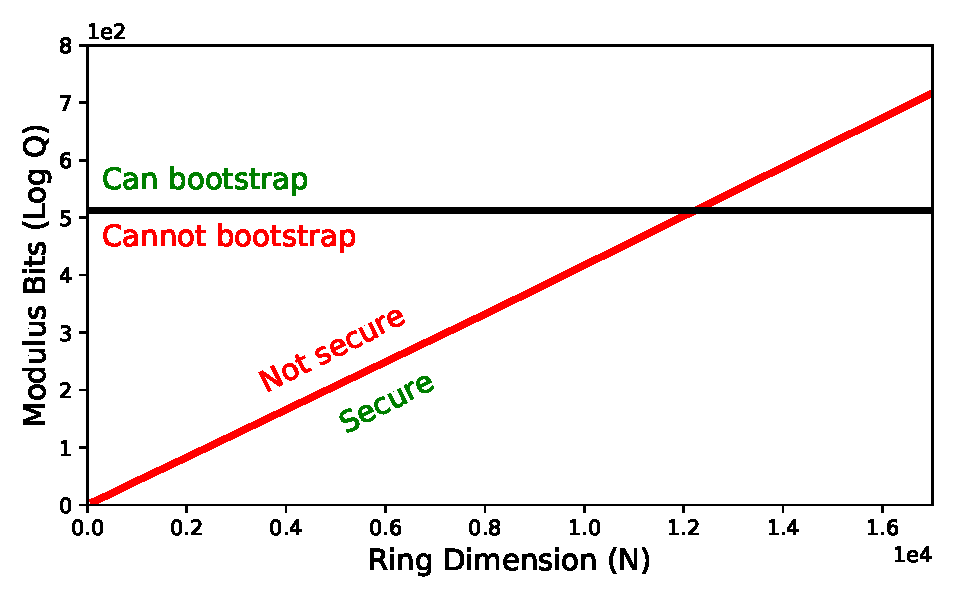
\includegraphics[width=0.75\columnwidth]{plots/security.pdf}
    \caption{Trade-offs between FHE parameters. Parameter values above the
      red line are deemed insecure (i.e., correspond to a security parameter below $80$ bits). The
      parameter values below the black line do not allow for bootstrapping.}
    \label{fig:paramTradeoffs}
    \vspace{-0.03in}
    \end{center}
  \end{figure}
}

\newcommand{\figArch}{
  \begin{figure}[h]
        \begin{center}
     \includegraphics[width=\columnwidth]{figures/ag_arch.pdf}
     \vspace{-0.12in} % this negative vspace... adds space  (which is what I want)
     \caption{Overview of the \name architecture.}
     \vspace{0.025in} % leave bottoms flush
    \label{fig:arch}
  \end{center}
  \end{figure}
}

\newcommand{\figMultDataflow}{
  \begin{figure}[h]
        \begin{center}
     \includegraphics[width=0.99\columnwidth]{figures/ag_mult_dataflow.pdf}
    \caption{Example matrix-vector multiply using FHE.}
    \label{fig:MultDataflow}
    \vspace{-0.1in}
    \end{center}
  \end{figure}
}

\newcommand{\figOpBreakdown}{
    \begin{figure}[h]
    \begin{center}
        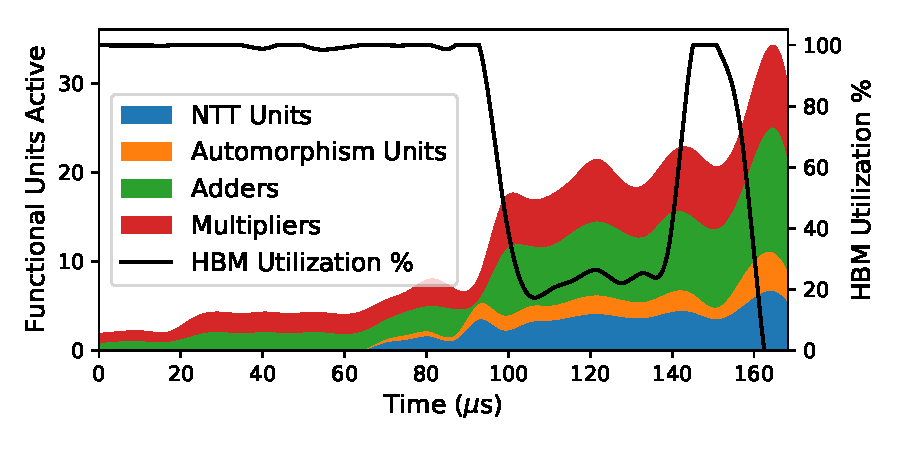
\includegraphics[width=0.7\columnwidth]{plots/lolaptwTimeplot.pdf}
        \caption{Functional unit and HBM utilization over time for the LoLa-MNIST PTW benchmark.}
        \label{fig:opBreakdown}
    \end{center}
    \end{figure}
}

\newcommand{\figCompilerOverview}{
  \begin{figure}[h]
        \begin{center}
     \includegraphics[width=\columnwidth]{figures/ag_compiler_overview.pdf}
    \caption{Overview of the \name compiler.}
    \label{fig:compilerOverview}
    %\vspace{-0.06in} %dsm: Shaves off a line, but looks bad
    \end{center}
  \end{figure}
}

\newcommand{\figautfu}{
\setlength{\columnsep}{7pt}
  \begin{figure}[h]
    \begin{center}
      \vspace{-0.8em}
     \includegraphics[width=0.25\columnwidth]{figures/ag_aut_fu.pdf}
    \caption{Automorphism unit.}
    \label{fig:aut_fu}
    \vspace{-0.4em} 
    \end{center}
  \end{figure}
}

\newcommand{\figAutomorphism}{
  \begin{figure}[h]
        \begin{center}
    \includegraphics[width=0.99\columnwidth]{figures/ag_automorphism.pdf}
    \caption{Applying $\sigma_3$ on a ciphertext of four 4-element chunks by using only permutations local to chunks.}
    \label{fig:automorphism}
    \end{center}
  \end{figure}
}

\newcommand{\figTranspose}{
  \begin{figure}[h]
    \centering
    \includegraphics[width=0.5\columnwidth]{figures/ag_transpose.pdf}
    \caption{The transpose unit.}
    \label{fig:transpose}
  \end{figure}
}

\newcommand{\figFourStepNTT}{
  \begin{figure}[h]
    \includegraphics[width=0.99\columnwidth]{figures/ag_four_step_ntt.pdf}
    \caption{Example of a four-step NTT datapath that uses 4-point NTTs to implement 16-point NTTs.}
    \label{fig:fourStepNTT}
    \vspace{1em}
  \end{figure}
}

\newcommand{\figQuadrantSwap}{
  \begin{figure}[h]
    \centering
    \includegraphics[width=0.75\columnwidth]{figures/ag_quadrant_swap.pdf}
    \caption{Transpose unit (right) and its component quadrant-swap unit (left).}
    \label{fig:quadrantSwap}
    \vspace{0.1in}
  \end{figure}
}

\newcommand{\figOverview}{
  \begin{figure}[h]
    \centering
    \vspace{-0.11in}
    \includegraphics[width=.8\columnwidth]{figures/ag_overview.pdf}
    \caption{FHE allows a user to securely offload computation to an untrusted server.}
    %old: \caption{Workflow showing how FHE is used to securely offload computation to an untrusted server.}
    \label{fig:overview}
    \vspace{0.2cm}
  \end{figure}
}

\newcommand{\figFUSweep}{
  \begin{figure}[h]
        \begin{center}
     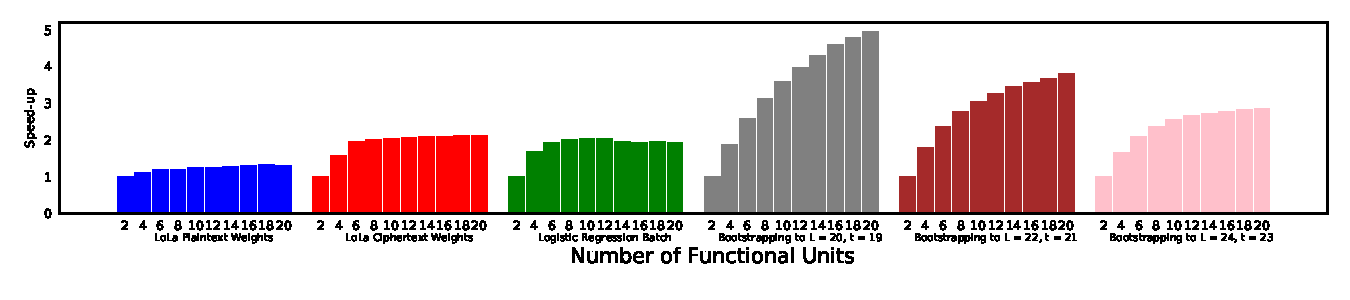
\includegraphics[width=\columnwidth]{plots/sweepFUs.pdf}
    \caption{Performance of our benchmarks with varying number of functional unit clusters.}
    \label{fig:sweepFUs}
    \vspace{-0.03in}
    \end{center}
  \end{figure}
}

\newcommand{\figBWSweep}{
  \begin{figure}[h]
        \begin{center}
     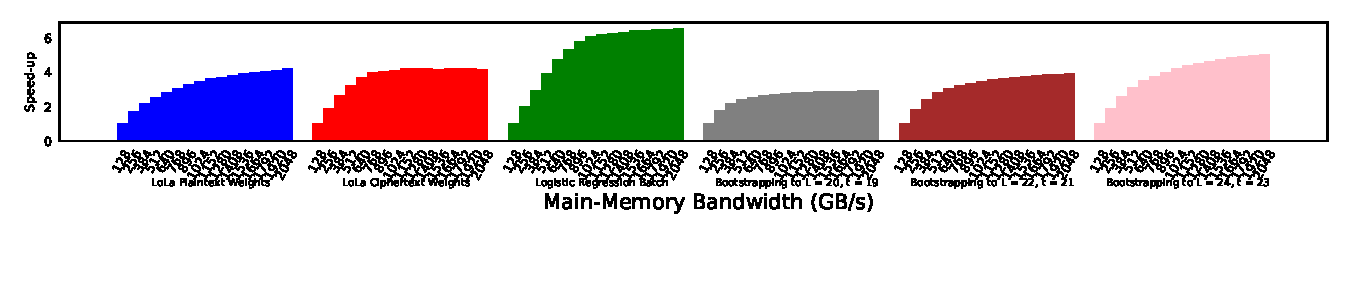
\includegraphics[width=\columnwidth]{plots/sweepBW.pdf}
    \caption{Performance of our benchmarks across various main memory bandwidths.}
    \label{fig:sweepBW}
    \vspace{-0.03in}
    \end{center}
  \end{figure}
}

\newcommand{\figDataMovement}{
\begin{figure}
  \centering
  \subfloat[]{
    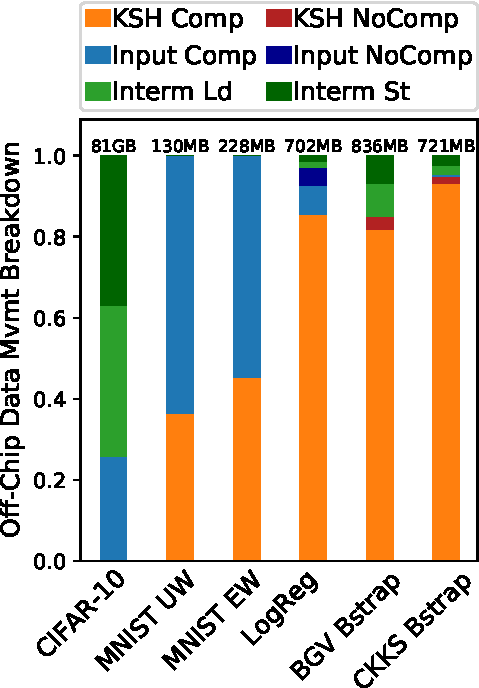
\includegraphics[width=0.4\linewidth]{plots/dataMovement.pdf}
    \label{fig:dataMovement}
  }
  \subfloat[]{
    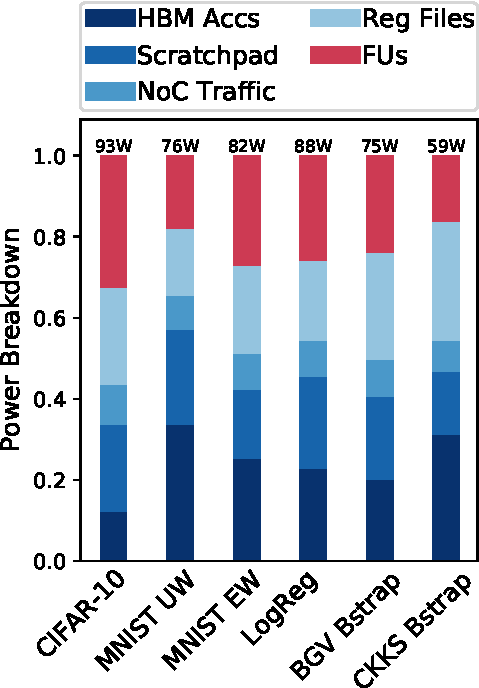
\includegraphics[width=0.4\linewidth]{plots/power.pdf}
    \label{fig:power}
  }
  \caption{Per-benchmark breakdowns of \textbf{(a)} data movement and \textbf{(b)} average power for \name.}
  %\vspace{0.1in}
\end{figure}
}

\newcommand{\figConfigs}{
    % \setlength{\columnsep}{7pt}
  \begin{figure}[h]
    % \vspace{-0.55in}
    \begin{center}
     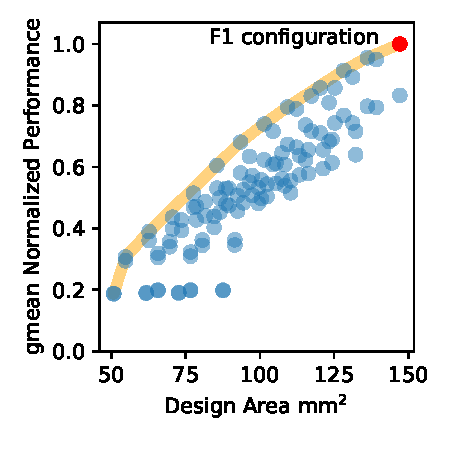
\includegraphics[width=0.45\columnwidth]{plots/configs.pdf}
    % \vspace{-0.26in}
    \caption{Performance vs. area across \name configurations.}
    \label{fig:pareto}
    % \vspace{-18pt}
    % \hspace{-0.03in}
    \end{center}
  \end{figure}
}

\newcommand{\figScratchpadSweep}{
  \begin{figure}[h]
        \begin{center}
     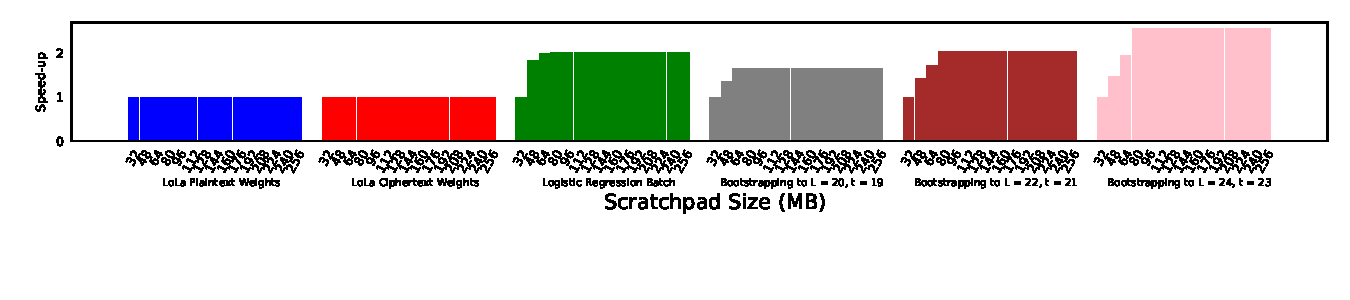
\includegraphics[width=\columnwidth]{plots/sweepScratchpad.pdf}
    \caption{Performance of our benchmarks across various scratchpad sizes.}
    \label{fig:sweepScratchpad}
    \vspace{-0.03in}
    \end{center}
  \end{figure}
}

\newcommand{\tblGF}{
  \begin{table}[h]
    \begin{center}
      \begin{footnotesize}
        \begin{tabular}{lrrr}
          \toprule
          Component & Area [mm$^2$] & TDP [W] \\
          \midrule
          NTT FU & 2.27 & 4.80  \\
          Automorphism FU & 0.58 & 0.99  \\
          %Transpose & 0.28 & \tmp{???} & - \\
          Multiply FU & 0.25 & 0.60  \\
          Add FU & 0.03 & 0.05  \\
          Vector RegFile (512\,KB) & 0.56 & 1.67 \\
          \textbf{Compute cluster} & 3.97 & 8.75 \\
          (NTT, Aut, 2$\times$ Mul, 2$\times$ Add, RF) & & \\
          \textbf{Total compute} (16 clusters) &  \textbf{63.52} & \textbf{140} \\
          \midrule
          Scratchpad (16$\times$4\,MB banks) & 48.09 & 20.35 \\
          3$\times$NoC (16$\times$16 512\,B bit-sliced~\cite{passas:tocaid12:crossbar}) & 10.02 & 19.65 \\
          Memory interface (2$\times$HBM2 PHYs) & 29.8 & 0.45 \\
          \textbf{Total memory system} &  \textbf{87.91} & \textbf{40.45} \\
          \midrule
          \textbf{Total \name} &  \textbf{151.43} & \textbf{180.45} \\
          \bottomrule
        \end{tabular}
      \end{footnotesize}
    \end{center}
    \vspace{-0.08in}
    \caption{Area and Thermal Design Power (TDP) of \name, and breakdown by component.}
    \label{tbl:GF12}
    \vspace{-0.1in}
  \end{table}
}


\newcommand{\tblNomenclature}{
   \begin{table}[h]
     \begin{footnotesize}
        \begin{center}
           \begin{tabular}{ll}
              \toprule
              \textbf{Param} & \textbf{Definition} \\
              \midrule
               \multicolumn{2}{c}{FHE Parameters} \\
              \midrule
              $N$ & Number of vector elements / polynomial coefficients \\
              $Q$ & Ciphertext modulus \\
              $t$ & Plaintext modulus \\
              \midrule
               \multicolumn{2}{c}{Architecture Parameters} \\
              \midrule
              $L$ & Number of RNS polynomials per ciphertext polynomial \\
              $q_i$ & The $i$-th RNS modulus ($Q = q_0q_1...q_{L-1}$) \\
              $E$ & Number of vector lanes \\
              $V$ & Vector operation initiation interval ($V = N/E$) \\ % dsm: Chimes? I don't know of a good nomenclature for this...
              \bottomrule
           \end{tabular}
           \label{tbl:nomenclature}
        \end{center}
        \caption{Nomenclature of key parameters in this paper.}
     \end{footnotesize}
   \end{table}
}

\newcommand{\tblModMult}{
  \begin{table}[h]
    \begin{footnotesize}
      \begin{center}
        \begin{tabular}{lrrr}
          \toprule
          Multiplier & Area [$\mu$m$^2$] & Power [mW] & Delay [ps] \\
          \midrule
          Barrett & $5,271$ & $18.4$ & 1,317 \\
          Montgomery & $2,916$ & $9.2$ & 1,040 \\
          NTT-friendly & $2,165$ & $5.36$ & 1,000 \\ % assumes q = 2^11m+1
          \midrule
          \textbf{FHE-friendly (ours)} & $1,817$ & $4.1$ & 1,000 \\
          \bottomrule
        \end{tabular}
        \vspace{0.02in}
        \caption{Area, power, and delay of modular multipliers.}
        \label{tbl:modMult}
      \end{center}
    \end{footnotesize}
    \vspace{-0.18in}
  \end{table}
}

\newcommand{\x}{$\times$}


\newcommand{\tblMicrobenchmark}{
  \begin{table}[t]
      % \vspace{-0pt}
      \begin{center}
      \resizebox{\columnwidth}{!}{%
      \begin{tabular}{l|rrr|rrr|rrr}
        \toprule
        & \multicolumn{3}{c|}{$N = 2^{12}$, $\log Q = 109$} &
        \multicolumn{3}{c|}{$N = 2^{13}$, $\log Q = 218$} &
        \multicolumn{3}{c}{$N = 2^{14}$, $\log Q = 438$} \\
        
        & \textbf{\name} & vs.\ CPU & vs.\ HEAX$_\sigma$ & \textbf{\name} & vs.\ CPU & vs.\ HEAX$_\sigma$ & \textbf{\name} & vs.\ CPU & vs.\ HEAX$_\sigma$\\

        \midrule

        % --- NTT

        % N=2**12, logQ = 109
        NTT
        &\textbf{12.8} % our
        &17,148$\times$ % CPU
        &1,600$\times$ % HEAX

        % N=2**13, logQ = 218
        &\textbf{44.8} % our
        &10,736$\times$ % CPU
        &1,733$\times$ % HEAX

        % N=2**14, logQ = 438
        &\textbf{179.2} % our
        &8,838$\times$ % CPU
        &1,866$\times$ % HEAX
        \\
        % --- Automorph. w/out k-s
        
        % N=2**12, logQ = 109
        Automorphism 
        &\textbf{12.8} % our
        &7,364$\times$ % CPU
        &440$\times$ % HEAX

        % N=2**13, logQ = 218   
        &\textbf{44.8} % our
        &8,250$\times$ % CPU
        &426$\times$ % HEAX

        % N=2**14, logQ = 438
        &\textbf{179.2} % our
        &16,957$\times$ % CPU
        &430$\times$ % HEAX
        \\

        \midrule

        % --- Ctxt-Ctxt Mult.

        % N=2**12, logQ = 109    
        Homomorphic multiply
        &\textbf{60} % our - % 60 MULS * 32 * 1/(32) = 60 cycles
        &48,640$\times$ % CPU
        &172$\times$ % HEAX

        % N=2**13, logQ = 218
        &\textbf{300} % our
        &27,069$\times$ % CPU
        &148$\times$ % HEAX

        % N=2**14, logQ = 438
        &\textbf{2,000} % our
        &14,396$\times$ % CPU
        &190$\times$ % HEAX
        \\

        % --- Automorph. w/ k-s

        % N=2**12, logQ = 109    
        Homomorphic permutation
        &\textbf{40} % our
        &17,488$\times$ % CPU
        &256$\times$ % HEAX

        % N=2**13, logQ = 218
        &\textbf{224} % our
        &10,814$\times$ % CPU
        &198$\times$ % HEAX

        % N=2**14, logQ = 438
        &\textbf{1,680} % our
        &6,421$\times$ % CPU
        &227$\times$ % HEAX
        \\
        
        \bottomrule
      \end{tabular}
      }
      %}
      \end{center}
      %\vspace{-5pt}
      \caption{Performance on microbenchmarks: \name's \textbf{reciprocal throughput, in nanoseconds per ciphertext operation} (lower is better) and speedups over CPU and HEAX$_\sigma$ (HEAX augmented with scalar automorphism units) (higher is better).}
      \label{tbl:microbenchmark}
      %\vspace{-3pt} % dsm: Leaves flush with other pages
  \end{table}
    % dsm: Now explained in text
    %\footnotetext[2]{We assume an SRAM array is used to perform an automorphism via random reads because HEAX does not report how they implement automorphisms.}
    %     \footnotetext[3]{We assume throughput is bottleneck on either the automorphism or keyswitching throughput, whichever is smaller.}
}


\newcommand{\tblBenchmark}{
  \begin{table}[t]
    \begin{footnotesize}
      \begin{center}
      \begin{tabular}{lrrr}
        \toprule
        Execution time (ms) on & CPU & \name & Speedup \\
        
        \midrule
        LoLa-CIFAR Unencryp. Wghts. & $1.2\times10^6$ & \textbf{241} & $5,011$\x \\
        LoLa-MNIST Unencryp. Wghts. & $2,960$ & \textbf{0.17} & $17,412$\x \\
        LoLa-MNIST Encryp. Wghts. & $5,431$ & \textbf{0.36} & $15,086$\x \\
        Logistic Regression & $8,300$ & \textbf{1.15} & $7,217$\x \\
        BGV Bootstrapping & ---\footnotemark[2] & \textbf{1.8} & ---\footnotemark[2] \\  % L=24
        CKKS Bootstrapping & $1,554$ & \textbf{1.3} & $1,195$\x \\    % L=24
        \midrule

        \textbf{gmean speedup} &&& 6,471\x \\
        % CKKS Bootstrapping $L=22$ & $1456$ & \textbf{2.2} & $662$\x \\
        % CKKS Bootstrapping $L=20$ & $1314$ & \textbf{1.9} & $692$\x \\
        \bottomrule
      \end{tabular}
   \end{center}
    \vspace{-8pt}
      \hfill\footnotemark[1]{LoLa's release did not include MNIST with encrypted weights, so we reimplemented it in HELib.}\quad\mbox{} \\
      \hfill\footnotemark[2]{BGV bootstrapping in HELib crashes for this input, and we could not find an alternative implementation or fix HELib. We expect \name's speedup to be at least 3,000$\times$}.\quad\mbox{}
    \end{footnotesize}
    \vspace{4pt}
      \caption{Performance of \name and CPU on full FHE benchmarks: execution times in milliseconds
      and \name's speedup.}      
      \label{tbl:benchmark}
      \vspace{-6pt}
  \end{table}
}

\newcommand{\tblPrimitiveOps}{
  \begin{table}[h]
    \begin{footnotesize}
      \begin{center}
        \caption{Operations in BGV \cite{}, CKKS \cite{}, and GSW \cite{} schemes and their constituent
        \textit{primitive operations}, which \name FUs acelerate. BGV and CKKS use very similar FHE operations
        and differ mainly in encryption/decryption.}
        \begin{tabular}{l|rr}
          \toprule
          & \multicolumn{2}{c}{\textbf{Required primitive operations}} \\
          \textbf{Operation} & \textbf{BGV/CKKS} & \textbf{GSW} \\
          \midrule
          Ciphertext add & add & add \\
          Ciphertext mult & NTT, mult & NTT, mult, add \\
          Key switching/relin & NTT, mult, add & N/A \\
          Mod switching & NTT, reduce, add & NTT, reduce, add \\
          Bootstrapping & automorphism, all ops & automorphism, all ops \\
          \bottomrule
        \end{tabular}
        \label{tbl:primitiveOps}
      \end{center}
    \end{footnotesize}
  \end{table}
}

\newcommand{\cipher}{\textsf{Ciphertext}}
\newcommand{\plain}{\textsf{Plaintext Vector}}
\newcommand{\scalar}{\textsf{Plaintext Scalar}}

\newcommand{\tblDSLOps}{
  \begin{table}[h]
    \begin{footnotesize}
      \begin{center}
        \caption{Supported FHE Operations and Types}
        \begin{tabular}{l|r}
            \textbf{Operation} & \textbf{Type}\\
            \midrule
            \textsf{Mul} & $\cipher \times \cipher \rightarrow \cipher$ \\
            \textsf{MulPlaintext} & $\cipher \times \plain \rightarrow \cipher$ \\
            \textsf{MulScalar} & $\cipher \times \scalar \rightarrow \cipher$ \\
            \textsf{Add} & $\cipher \times \cipher \rightarrow \cipher$ \\
            \textsf{AddPlaintext} & $\cipher \times \plain \rightarrow \cipher$ \\
            \textsf{AddScalar} & $\cipher \times \scalar \rightarrow \cipher$ \\
            \textsf{Rotate} & $\cipher \times \scalar \rightarrow \cipher$ \\
            \textsf{ModDown} & $\cipher \times \scalar \rightarrow \cipher$ \\
        \end{tabular}
      \end{center}
    \end{footnotesize}
  \end{table}
}


\newcommand{\tblSensitivity}{
  \begin{table}[h]
    \begin{footnotesize}
      \begin{center}
        \begin{tabular}{lrrr}
            \toprule
            Benchmark & LT NTT & LT Aut & CSR \\
            \midrule
            LoLa-CIFAR Unencryp. Wghts. & 3.5\x & 12.1\x & ---\footnotemark[1] \\
            LoLa-MNIST Unencryp. Wghts. & 5.0\x & 4.2\x & 1.1\x \\
            LoLa-MNIST Encryp. Wghts. & 5.1\x & 11.9\x & 7.5\x \\
            Logistic Regression & 1.7\x & 2.3\x & 11.7\x \\
            BGV Bootstrapping & 1.6\x & 1.1\x & 5.4\x \\
            CKKS Bootstrapping & 1.1\x & 1.2\x & 2.7\x \\
            \midrule
            \textbf{gmean speedup} & 2.5\x & 5.5\x & 4.2\x \\
            \bottomrule
        \end{tabular}
      \end{center}
      \vspace{-8pt}
      \hfill\footnotemark[1]{CSR is intractable for this benchmark.}\quad\mbox{}
    \end{footnotesize}
    \vspace{4pt}
        \caption{Speedups of \name over alternate configurations: %without our contributions:
          LT NTT/Aut = Low-throughput NTT/Automorphism FUs; CSR = Code Scheduling to minimize Register Usage \cite{goodman:ics1988:code}.}
        \label{tbl:sensitivity}
    \vspace{-2pt}
  \end{table}
}

\newcommand{\C}{\textsf{Scalar}}
\newcommand{\V}{\textsf{Vector}}
\newcommand{\q}{\textsf{Modulus}}

\newcommand{\tblISA}{
  \begin{table}[h]
  \begin{footnotesize}
  \begin{center}
  \caption{\name ISA}
  \begin{tabular}{lr}
  \toprule
  Instruction & Type \\
  \midrule
  \texttt{ADD} & $\V \times \V \times \q \rightarrow \V$ \\
  \texttt{ADD\_SCALAR} & $\V \times \C \times \q \rightarrow \V$ \\
  \texttt{MUL} & $\V \times \V \times \q \rightarrow \V$ \\
  \texttt{MUL\_SCALAR} & $\V \times \C \times \q \rightarrow \V$ \\
  \texttt{NTT} & $\V \times \q \rightarrow \V$ \\
  \texttt{INTT} & $\V \times \q \rightarrow \V$ \\
  \texttt{AUTOMORPHISM} & $\V \times \C \rightarrow \V$ \\
  \end{tabular}
  \label{tbl:isa}
  \end{center}
  \end{footnotesize}
  \end{table}
}



%% This bit allows you to either specify only the files which you wish to
%% process, or `all' to process all files which you \include.
%% Krishna Sethuraman (1990).

%\typein [\files]{Enter file names to process, (chap1,chap2 ...), or `all' to
%process all files:}
%\def\all{all}
%\ifx\files\all \typeout{Including all files.} \else \typeout{Including only \files.} \includeonly{\files} \fi

\begin{document}

% -*-latex-*-
% 
% For questions, comments, concerns or complaints:
% thesis@mit.edu
% 
%
% $Log: cover.tex,v $
% Revision 1.8  2008/05/13 15:02:15  jdreed
% Degree month is June, not May.  Added note about prevdegrees.
% Arthur Smith's title updated
%
% Revision 1.7  2001/02/08 18:53:16  boojum
% changed some \newpages to \cleardoublepages
%
% Revision 1.6  1999/10/21 14:49:31  boojum
% changed comment referring to documentstyle
%
% Revision 1.5  1999/10/21 14:39:04  boojum
% *** empty log message ***
%
% Revision 1.4  1997/04/18  17:54:10  othomas
% added page numbers on abstract and cover, and made 1 abstract
% page the default rather than 2.  (anne hunter tells me this
% is the new institute standard.)
%
% Revision 1.4  1997/04/18  17:54:10  othomas
% added page numbers on abstract and cover, and made 1 abstract
% page the default rather than 2.  (anne hunter tells me this
% is the new institute standard.)
%
% Revision 1.3  93/05/17  17:06:29  starflt
% Added acknowledgements section (suggested by tompalka)
% 
% Revision 1.2  92/04/22  13:13:13  epeisach
% Fixes for 1991 course 6 requirements
% Phrase "and to grant others the right to do so" has been added to 
% permission clause
% Second copy of abstract is not counted as separate pages so numbering works
% out
% 
% Revision 1.1  92/04/22  13:08:20  epeisach

% NOTE:
% These templates make an effort to conform to the MIT Thesis specifications,
% however the specifications can change.  We recommend that you verify the
% layout of your title page with your thesis advisor and/or the MIT 
% Libraries before printing your final copy.
\title{Enabling Real-time Private DNN Inference Using Fully Homomorphic Encryption}

\author{Nikola Samardzic}
% If you wish to list your previous degrees on the cover page, use the 
% previous degrees command:
%       \prevdegrees{A.A., Harvard University (1985)}
% You can use the \\ command to list multiple previous degrees
%       \prevdegrees{B.S., University of California (1978) \\
%                    S.M., Massachusetts Institute of Technology (1981)}
\prevdegrees{B.S. in Computer Science\linebreak
University of California, Los Angeles, 2020}
\department{Electrical Engineering and Computer Science}

% If the thesis is for two degrees simultaneously, list them both
% separated by \and like this:
% \degree{Doctor of Philosophy \and Master of Science}
\degree{Master of Science in Electrical Engineering and Computer Science}

% As of the 2007-08 academic year, valid degree months are September, 
% February, or June.  The default is June.
\degreemonth{May}
\degreeyear{2022}
\thesisdate{May 13, 2022}

%% By default, the thesis will be copyrighted to MIT.  If you need to copyright
%% the thesis to yourself, just specify the `vi' documentclass option.  If for
%% some reason you want to exactly specify the copyright notice text, you can
%% use the \copyrightnoticetext command.  
%\copyrightnoticetext{\copyright IBM, 1990.  Do not open till Xmas.}

% If there is more than one supervisor, use the \supervisor command
% once for each.
\supervisor{Daniel Sanchez}{Associate Professor of Electrical Engineering and Computer Science}

% This is the department committee chairman, not the thesis committee
% chairman.  You should replace this with your Department's Committee
% Chairman.
\chairman{Leslie A. Kolodziejski}{
Professor of Electrical Engineering and Computer Science\\
Chair, Department Committee on Graduate Students}

% Make the titlepage based on the above information.  If you need
% something special and can't use the standard form, you can specify
% the exact text of the titlepage yourself.  Put it in a titlepage
% environment and leave blank lines where you want vertical space.
% The spaces will be adjusted to fill the entire page.  The dotted
% lines for the signatures are made with the \signature command.
\maketitle

% The abstractpage environment sets up everything on the page except
% the text itself.  The title and other header material are put at the
% top of the page, and the supervisors are listed at the bottom.  A
% new page is begun both before and after.  Of course, an abstract may
% be more than one page itself.  If you need more control over the
% format of the page, you can use the abstract environment, which puts
% the word "Abstract" at the beginning and single spaces its text.

%% You can either \input (*not* \include) your abstract file, or you can put
%% the text of the abstract directly between the \begin{abstractpage} and
%% \end{abstractpage} commands.

% First copy: start a new page, and save the page number.
\cleardoublepage
% Uncomment the next line if you do NOT want a page number on your
% abstract and acknowledgments pages.
% \pagestyle{empty}
\setcounter{savepage}{\thepage}
\begin{abstractpage}

\emph{``This innovation that this industry talks about so much is bullshit. Anybody
can innovate. Don't do this `think different'; don't do this big `innovation'
thing. Screw that. It's meaningless. 99\% of it is: get the work done.''}

--- Linus Torvalds
\vspace{1cm}

Fully Homomorphic Encryption (FHE) allows computing on encrypted data, enabling secure offloading of computation to untrusted servers.
Though it provides ideal security, FHE is expensive when executed in software, 4 to 5 orders of magnitude slower than computing on unencrypted data.
These overheads are a major barrier to FHE's widespread adoption.

We present \name, the first FHE accelerator that is programmable, i.e., capable of executing full FHE programs.
\name builds on an in-depth architectural analysis of the characteristics of FHE computations
that reveals acceleration opportunities. \name is a wide-vector processor with novel functional units deeply specialized to FHE primitives, 
such as modular arithmetic, number-theoretic transforms, and structured permutations.

% axelf: tentative?
Due to the static nature of FHE computations, \name uses an exposed ISA, requiring novel compilation techniques to statically schedule all compute and data movement. We design a compiler that efficiently maps FHE programs onto \name hardware and maximizes reuse of on-chip data, helping to reduce data movement bottlenecks. 
The compiler leverages \name's explicitly managed scratchpad to decouple computation from data movement, a necessary ingredient in achieving high performance given the large size of FHE operands.

% This organization provides so much compute throughput that data movement becomes the key bottleneck.
% Thus, \name is primarily designed to minimize 
% data movement.
% Hardware provides an explicitly-managed memory hierarchy and mechanisms to decouple data movement from execution.
% A novel compiler leverages these mechanisms to maximize reuse and schedule off-chip and on-chip data movement.
 
We evaluate \name using cycle-accurate simulation and RTL synthesis.
\name is the first system to accelerate complete FHE programs,
and outperforms state-of-the-art software implementations by gmean 6,500$\times$ and by up to 17,000$\times$.
These speedups counter most of FHE's overheads and enable new applications, like real-time private deep learning in the cloud.

\end{abstractpage}

% Additional copy: start a new page, and reset the page number.  This way,
% the second copy of the abstract is not counted as separate pages.
% Uncomment the next 6 lines if you need two copies of the abstract
% page.
% \setcounter{page}{\thesavepage}
% \begin{abstractpage}
% % $Log: abstract.tex,v $
% Revision 1.1  93/05/14  14:56:25  starflt
% Initial revision
% 
% Revision 1.1  90/05/04  10:41:01  lwvanels
% Initial revision
% 
%
%% The text of your abstract and nothing else (other than comments) goes here.
%% It will be single-spaced and the rest of the text that is supposed to go on
%% the abstract page will be generated by the abstractpage environment.  This
%% file should be \input (not \include 'd) from cover.tex.



% \end{abstractpage}

\cleardoublepage

\section*{Acknowledgments}

Thank you to all the people that created the environment in which success is
easy. Your work matters and changes lives.

This work was conducted in collaboration with Axel Feldmann, Aleksandar
Krastev, Nicholas Genise, Prof. Srini Devadas, Karim Eldefrawy, Nathan Manohar,
Prof. Ron Dreslinski, Prof. Chris Peikert, and my research advisor Prof. Daniel
Sanchez. Much of this thesis is adapted from joinly written papers. This work
would not have been possible without all of their contributions.


%%%%%%%%%%%%%%%%%%%%%%%%%%%%%%%%%%%%%%%%%%%%%%%%%%%%%%%%%%%%%%%%%%%%%%
% -*-latex-*-

% Some departments (e.g. 5) require an additional signature page.  See
% signature.tex for more information and uncomment the following line if
% applicable.
% \include{signature}
\pagestyle{plain}
  % -*- Mode:TeX -*-
%% This file simply contains the commands that actually generate the table of
%% contents and lists of figures and tables.  You can omit any or all of
%% these files by simply taking out the appropriate command.  For more
%% information on these files, see appendix C.3.3 of the LaTeX manual.
\tableofcontents
\newpage
%\listoffigures
%\newpage
%\listoftables


\section{Introduction}\label{sec:intro}

A large and increasing fraction of the world's compute runs on the cloud,
which is vulnerable to data breaches.
Conventional techniques to mitigate attacks offer limited 
security, as cloud servers must decrypt data in order to process it.

\emph{Fully homomorphic encryption (FHE)} is a special type of encryption scheme
that enables \emph{computing on encrypted data directly}, without decrypting it.
FHE allows a client to offload a computation
to an untrusted server \emph{without} revealing any data (\autoref{fig:workflow}).
This enables the client to harness the compute power of the cloud while maintaining cryptographic privacy.
Though FHE has some limitations (e.g., data-dependent branching is not possible), 
it is general enough to support many compelling use cases,
such as privacy-preserving machine learning, secure genome analysis, private set intersection,
private information retrieval, and many more~\cite{kim2020semi,gilad:icml16:cryptonets,han:aaai19:logistic,han:iacr18:efficient,juvekar2018gazelle,DBLP:conf/ccs/ChenLR17,DBLP:conf/tcc/GentryH19}. 
%\nnote{add citations and more examples}

% axelf: purging unfortunately/fortunately from the whole paper
Despite its ideal privacy, FHE is rarely used today because it incurs prohibitive overheads:
in CPUs, FHE computations are 10,000$\times$ to 100,000$\times$
slower than equivalent unencrypted computations, even when using highly optimized FHE libraries.
% dsm: I don't think this adds much here, other than distance to get to the actual point
%Some of these overhead costs are due
%to the size of FHE ciphertexts while
%others are due to the additional complexity
%of representing arbitrary functions in a form suitable for
% computing using FHE.

Fortunately, state-of-the-art FHE schemes are well-suited to hardware acceleration.
First, they are regular and structured:
FHE programs operate on very long vectors, and all operations are known ahead of time.
Second, FHE requires several non-SIMD operations,
such as \emph{number-theoretic transforms} (NTTs),
that are inefficient on CPUs and GPUs.
But these operations can be accelerated by specialized functional units,
avoiding these inefficiencies.
As a result, prior work has proposed FPGA and ASIC-based
accelerators~\cite{riazi:asplos20:heax,cousins:hpec12:sipher-fpga,cousins:tetc17:fpga-he,turan:tc20:heaws,cousins:hpec14:fpga-he, roy:hpca19:fpga-he,feldmann:micro21:f1}.
While most prior accelerators achieve limited speedups, a recent design,
F1~\cite{feldmann:micro21:f1}, achieves speedups of
%2,000-15,000$\times$ 
% dsm: Let's avoid the 15000x speedup, we don't have anything that large but we're using a different baseline, diff configs, etc.
about 5,000$\times$
on FHE programs.

% dsm: Unfortunately here is important. We were just describing potential, we want to signpost that we're entering negative territory.
Unfortunately, prior accelerators are efficient only on a limited subset of simple FHE
computations---those of \emph{shallow multiplicative depth}.
% FIXME(dsm): I think this may be from edits, but right now several terms are left undefined: DEPTH and MULTIPLICATIVE DEPTH. I think this is because the text below does not talk about multiplications.
For example, prior FHE accelerators can run neural network inference efficiently only for networks with few layers (3-6),
but they cannot accelerate state-of-the-art deep neural networks (DNNs) with tens to hundreds of layers.

This limitation stems from the characteristics of FHE schemes:
each ciphertext has some associated noise, which grows with each homomorphic operation, and especially with multiplications.
If noise becomes too large, it garbles the message, making decryption impossible. 
%To support computations with higher multiplicative depth, the size of ciphertexts must increase to counteract the additional noise growth, resulting in each FHE operation being more computationally expensive.
Larger ciphertexts tolerate more noise before becoming undecryptable. 
However, operations on larger ciphertexts are also more expensive.
To enable computations of unbounded depth, ciphertexts can be ``refreshed'' using a procedure called \emph{bootstrapping}
that reduces noise. But bootstrapping is expensive, 
% dsm: multiplicative depth is NOT YET DEFINED
%and itself consumes multiplicative depth, 
so ciphertexts must be very large (10s of MBs) for bootstrapping to be
efficient.

Prior FHE accelerators do not efficiently handle unbounded-depth computations because
they natively support vectors of a limited size and they use algorithms that scale poorly
to the large ciphertexts in high-depth programs.
As a result, they can only run small FHE computations, and they do not support sufficient depth
to run the full bootstrapping procedure.

\figWorkflow

In this paper we tackle this challenge through \name, the first FHE accelerator
to support \emph{FHE computations of unbounded depth}.
To achieve this, we contribute new algorithms, specialized functional units,
hardware architecture, and compiler techniques that overcome the key challenge
of deep FHE computations---its extreme data movement demands.

\paragraph{Deep FHE is limited by data movement:}
FHE schemes encode information over very long vectors of wide elements.
Concretely, supporting unbounded-depth computations requires vectors of
64K elements with 1,600 bits per element.
This takes 25\,MB per ciphertext, 12$\times$ larger than what prior FHE accelerators target.
% nikola; 25MB = 2 * 1600 bits * 64*1024 elements * (1/8) bytes / bit * 1/2^20 bytes / MB

% (alex): I changed the comparisson from to 32 MB to 23 MB ciphertexts;
%         Being charittable, this is L = 1500/32 = 46 for F1 and KSH is 23*46 = 1058MB
% nikola: 2MB ciphertext in F1 => 1MB per ciphertext polynomial => 512 bits per coeff at N=16K
% => L = 16 (32-bit moduli) => KSH = 2*L^2*N * 32 bits / elem = 32 MB
% nikola: 26MB ciphertext in F1 => 13MB per ciphertext polynomial + assume N=64K
% => log Q = 1,664 => L = 52 => KSH = 2*L^2*N * 32 bits / elem * (1/8) B/bit * 1/2^30 GB/B
% = 1.32 GB
% At the same log Q = 1,664, CL needs L = 1664/28 = 60: KSH = 2*2*L*N = 
% = 2*2 * 60 (L) * 64*1024 (N) * 28 bits / elem * (1/8) B/bit * 1/2^20 MB/B = 52.5 MB
% (note that L is actually 1668/26.7, but we divide by 28 to be consistent with the F1
% methodology, where we multiply by 32)
Moreover, prior work has employed FHE algorithms that require even larger amounts of auxiliary data.
For example, multiplying 2\,MB ciphertexts in F1~\cite{feldmann:micro21:f1} requires 32\,MB of auxiliary data,
and scaling their algorithm to 26\,MB ciphertexts would require over
1.3\,GB 
of auxiliary data---far too large to fit on-chip.
To tackle this challenge, our \emph{key insight} is to adopt an FHE
algorithm called \emph{boosted keyswitching} (\autoref{sec:keyswitching}) that eliminates most of the
auxiliary data,
% (alex): KSH it's 2 ciphertexts without PRG
reducing this overhead from 1.3\,GB to 52.5\,MB.
%We further reduce this overhead to 23\,MB by introducing a new functional unit that
%generates half of this auxiliary data on the fly, rather than fetching it from memory.
Boosted keyswitching also reduces computation costs.
However, this new algorithm is a poor match for prior accelerators:
it is dominated by simple operations where these designs have limited efficiency,
and makes poor use of the specialized functional units that prior designs leverage.

Beyond being inefficient, prior accelerators suffer from a hard-to-scale vector multicore architecture:
to support the needed non-SIMD operations with reasonable cost,
they implement multiple independent cores with narrower vector datapaths~\cite{feldmann:micro21:f1}.
However, this causes excessive inter-core communication,
and the high-bandwidth interconnect
needed grows superlinearly with the number of cores.


\paragraph{Deep FHE demands new hardware techniques:}
To tackle these challenges, we introduce the \emph{\name} architecture (\autoref{sec:overview}, \autoref{sec:architecture}),
the first FHE accelerator that achieves high performance on unbounded FHE programs.
\name is a wide-vector uniprocessor with specialized functional units.
The design is statically scheduled to leverage the regularity of FHE computations.
We contribute several new techniques that make this possible, including:
\begin{compactitem}
\item A new extremely wide (2,048 lanes) vector uniprocessor architecture that
    spreads each vector operation across the chip, departing from prior vector multicore architectures.
The uniprocessor approach reduces the number of concurrent operations, which minimizes footprint,
  reducing off-chip traffic, and simplifies the compiler.
\item An efficient implementation of the above architecture, which is challenging for non-SIMD FHE operations, NTTs and automorphisms,
  by decomposing these operations in a novel way that allows the use of a \emph{fixed transpose network} among physically distributed groups of lanes.
  This reduces on-chip data movement and interconnect cost over prior approaches.
\item A new functional unit that encapsulates the bulk of operations in boosted keyswitching, improving efficiency and enabling high utilization across ciphertexts of all sizes.
\item A new functional unit that generates half of the required auxiliary data on the fly (reducing overheads from 52\,MB to 26\,MB), saving on-chip storage and memory bandwidth.
\item A vector chaining technique that builds long FU pipelines to enable many concurrent operations with few register ports.
\end{compactitem}
To program \name, we develop a novel compiler (\autoref{sec:compiler}) that produces efficient code from high-level FHE programs.
The compiler schedules operations to maximize reuse, decouples data movement from computation,
and adapts the state-of-the-art bootstrapping algorithm to achieve high
utilization~\cite{bossuat:crypto21:efficient}.


We evaluate \name through a combination of simulation and RTL synthesis (to find its area and power).
We use a broad range of FHE benchmarks, including programs with high multiplicative depth
that require bootstrapping.
\name outperforms a scaled-up and improved version of the state-of-the-art FHE accelerator, F1, by gmean 
11.2$\times$ on these deep computations,
and is 4,600$\times$ faster than a 32-core CPU.
These speedups enable new use cases for FHE.
For example, deep neural networks like ResNet
% which takes tens of \emph{minutes} per inference on CPUs,
% nikola: again, it really takes tens of minutes, but that's cuz of hours algo improvements
% dsm: Let's not confuse the reader, we can mention that this used to be hours in the eval but saying hours to ms is comparing apples to oranges
take 23 minutes per inference on the CPU,
whereas \name achieves 250 \emph{milliseconds} per inference,
enabling real-time private deep learning.
% 23 minutes = 1.37694e+12 ns / (10^9*60) = 22.9 min
% 265 ms = 2.64245e+08 / (10^6) = 264 ms


\chapter{Background}\label{sec:background}
% \nikola{need to introduce the NTT somewhere in this section; probably after data representation}
% \nikola{need to define an automorphism in this section; probably when defining homomorphic rotation}
% \nnote{referring to CKKS as an FHE scheme even though it's only for approximate arithmetic... people sometimes complain about this}


% CKKS\footnote{named after the authors}~\cite{ckks}
% is an FHE scheme that supports encrypted computations on vectors of real numbers.
% CKKS ciphertexts are a pair of degree-$N$ polynomials with coefficients
% being large integers modulo some $Q$. Common parameter
% regimes include $N$ from $1K$ to $64K$ and $\log_2(Q)$
% from $1K$ to $2K$.
% Choosing $N$ and $Q$ for proper performance
% and security depends on the program you want to run, and is an active area of
% research~\cite{DBLP:conf/crypto/May21}.
% For this reason, we focus exclusively on optimizing
% the performance of CKKS, although our accelerator can also be
% used for other FHE schemes.


State-of-the-art % dsm: Unless this is TFHE jab, why? nikola: The point is that in theory there may exist yet-undiscovered FHE schemes that work really well but dont operate on encrypted vectors :P
FHE schemes implement operations on~\emph{encrypted vectors}.
The FHE ciphertexts in these schemes support several \emph{homomorphic operations}:
element-wise addition, element-wise multiplication, and cyclic rotations of vector elements.
Each homomorphic operation produces a ciphertext that, when decrypted,
produces the same result as if the operation had been performed on the unencrypted inputs.

Importantly, homomorphic operations have a different implementation from their unencrypted counterparts---for example,
a homomorphic multiplication is not implemented using element-wise multiplication
of the input ciphertexts, but a more complex
sequence of operations. Therefore, it is useful to differentiate between FHE's \emph{interface},
i.e., its supported plaintext datatypes and operations,
and its \emph{implementation},
i.e., the structure of ciphertexts and the implementation of homomorphic operations.

There are several FHE schemes, which mainly differ in their plaintext datatypes and the operations they support.
For example, BGV~\cite{brakerski:toct14:leveled} encodes vectors of integers modulo a constant,
whereas CKKS~\cite{cheon:ictaci17:homomorphic} encodes vectors of fixed-point numbers.
Despite the differences between these schemes, % all state-of-the-art FHE schemes
%use a similar format for ciphertexts, as they rely on the hardness of the same problem
%(LWE or ring-LWE~\cite{lyubashevsky:tact10:ideal}) to attain security.
%have similarities since they all rely on the hardness of learning with errors (LWE) or its ring variant (ring-LWE)~\cite{lyubashevsky:tact10:ideal} to attain security.
the commonalities in their underlying implementation~\cite{lyubashevsky:tact10:ideal}
make it possible for the same hardware to
accelerate many schemes
efficiently---\name supports CKKS, BGV, and GSW~\cite{gentry:crypto13:homomorphic}.
For concreteness, the rest of this section will focus only on CKKS as it
is the scheme best suited for machine learning tasks and has been the focus of
recent work in FHE algorithms~\cite{han:iacr18:efficient,lee:2021:privacy,gilad:icml16:cryptonets,podschwadt:2020:classification,dathathri:pldi19:chet,dathathri:pldi20:eva}.

\subsection{FHE Interface}

%State-of-the-art % dsm: Whatever, once was enough
FHE schemes implement operations on vectors of values.
In CKKS, each vector element is a \emph{fixed-point} complex number with a configurable number of bits.
(Programs that do not use complex arithmetic can zero out the imaginary part.)
% with a set number of quotient and mantissa bits. % nikola: confusing % dsm: why?
% nikola: this is confusing because it is the definition of fixed point.
% so why put it there? As a reminder? That's alright, but I would add "i.e." or
% something
% dsm: No, it is important because architects are used to thinking about FIXED FORMATS, like fp32, bfloat16, etc. We must say that the number of bits is configurable.

Since values are encrypted, FHE does not permit data-dependent branching or indirection.
Thus, all operations and dependencies are known ahead of time, and FHE programs can
be represented using \emph{static dataflow graphs}.

% nikola: regarding Daniel's note on arbitrarily vs relatively. It _is_ true
% that we can make computation arbitrarily precise (just add bits of precision!).
Homomorphic operations in CKKS include element-wise addition, element-wise multiplication,
and cyclic rotations.
While these operations are \emph{approximate} in CKKS, inducing a small and
controllable amount of error, this error can be made arbitrarily small at the
cost of reduced performance. % \nnote{this is only true for a priori bounded-depth computation, but i think it's fine to not mention this}
% dsm: Someone changed arbitrarily to relatively. Unless this error absolutely cannot be reduced beyond a non-zero threshold, please don't fudge it. I don't care that it's expensive and it's not done in practice. Digital logic is also expensive vs analog, and wasn't considered practical for a long time, yet here we are. I'm trying to distance this from the minefield thsat is approximate computing.
This error is acceptable in practice as machine learning applications
are insensitive to it.

FHE exposes a vector programming model with a restricted set of operations; in particular,
FHE does not provide access to individual vector elements.
This makes it challenging to implement some operations
that are trivial in plaintext:
For example,
implementing a convolutional layer of a neural network requires the careful
replication of filter weights.
The lack of non-linear functions introduces other difficulties.
For example, the ReLU activation function must be approximated
using a high-degree polynomial~\cite{lee:2021:precise}.
%
As a result, faithfully replicating deep neural networks in FHE,
as done by a recent ResNet implementation~\cite{lee:2021:privacy}, comes at a high compute cost.
However, recent work has proposed neural network structures that are optimized
for FHE and achieve higher performance while maintaining similar accuracy~\cite{brutzkus:icml19:low}.
We evaluate \name on both styles of neural networks.

Finally, not all data needs to be encrypted:
additions and multiplications are much cheaper in FHE if one of the operands is unencrypted.
This allows algorithms to trade privacy for performance.
For example, running a neural network using unencrypted weights is faster; it
still ensures the privacy of inputs and results, but does not
protect weights~\cite{brutzkus:icml19:low}.

\subsection{FHE Implementation}

% \nnote{some FHE schemes are actually quite different, so i changed the wording here a bit. also, GSW is kind of different from BGV and CKKS}
We now describe how CKKS represents and operates on encrypted data (i.e., ciphertexts);
other schemes (e.g., BGV) have a similar structure.

\paragraph{Encryption:} A ciphertext holds an encrypted vector of plaintext values.
To create a ciphertext, the vector of plaintext values is first encoded, or \emph{packed},
in a polynomial; this polynomial is then \emph{encrypted}.
CKKS packs a plaintext vector of $ n = N/2$ complex fixed-point numbers
into a degree-$(N-1)$ polynomial:
% dsm: Sinbce this modulus doesn;t show up anywhere else, and it's unclear how you would pick t to support fixed-point numbers, I'm killing it.
%with integer coefficients modulo a plaintext
%modulus $t$:
\begin{equation*}
    (c_0, c_1, ..., c_n) \xmapsto{pack} \mathfrak{m} = k_0 + k_1x + ... + k_{N-1}x^{N-1} %\in R_q
\end{equation*}
% NOTE(dsm): Do not call m a plaintext.
$\mathfrak{m}$ is then encrypted into a ciphertext. Each ciphertext consists of
% nikola: better to call these ct_0, ct_1 instead of p_0, p_1 cuz then the homomorphic add example makes more sense (i.e., ct. polys are named after the ciphertext + an index)
$\mathfrak{ct}_0, \mathfrak{ct}_1$---two \emph{ciphertext polynomials}
with coefficients modulo a \emph{ciphertext modulus} $Q$.
Specifically, we encrypt $\mathfrak{m}$
under a \emph{secret key} $\mathfrak{s}$
by sampling a uniformly random $\mathfrak{a}$
and a small \emph{error} $\mathfrak{e}$ ($\mathfrak{s}$, $\mathfrak{a}$, and $\mathfrak{e}$ are also polynomials):
% nikola: change the above remark to a footnote instead of writing \in R_Q because s and e are *just* polynomials, and a is actually in R_Q. This distinction doesnt matter for ISCA, so I just say they are all polynomials, which is correct. But saying they are all in R_Q would actually be incorrect, so I forgoe it
\begin{equation*}
    \mathfrak{m} \xmapsto{encrypt} \mathfrak{ct} = (\mathfrak{ct}_0, \mathfrak{ct}_1) = (\mathfrak{a}, \mathfrak{a}\cdot\mathfrak{s}+\mathfrak{e}+\mathfrak{m})
\end{equation*}
% dsm: Comment out if low on space... but we do use partially packed later on.
The above process produces a \emph{fully-packed} ciphertext, i.e., one
that encodes as many plaintext values as possible. It is possible
(though almost always less efficient) to pack~fewer~values,
producing a partially packed or unpacked (one-element) ciphertext.

% dsm: We need to be careful with how this is described, it seems like this is horribly approximate and the interface is already talking about the error. Positionaing this as approximate computing would be a strategic mistake.
%The noise term is necessary for the message $m$ to be cryptographically secure.
%Also, note how the message's low-order bits are corrupted by the error.
%This often does not interfere with the final computation
%since computations done with CKKS are convergent and CKKS's
%encoding mechanism accounts for the error-message interaction,
%i.e.\ the significant bits are encoded well above the error.
%The latter is because the noise growth in each FHE computation is predictable.


\paragraph{Homomorphic operations} are implemented through several modular-arithmetic operations on ciphertext polynomials, i.e., vectors of coefficients. Specifically:
\begin{compactitem}
\item \emph{Homomorphic addition} of two ciphertexts simply requires modular addition of their ciphertext polynomials:
    $\mathfrak{ct}_{\textrm{add}} = \mathfrak{a} + \mathfrak{b} = (\mathfrak{a}_0+\mathfrak{b}_0, \mathfrak{a}_1+\mathfrak{b}_1)$.
\item \emph{Homomorphic multiplication} is implemented using polynomial multiplications and additions;
  multiplying two polynomials requires convolving their coefficients.
% nikola: there was a convolving elements thing here... this is confusing. I would just say it this way.
% dsm: Nikola, the whole point is to make it crystal clear thea POLYNOMAIL MULTIPLICATION != MULTIPLICATION. Otherwise the NTT will ome as a complete surprise.
\item \emph{Homomorphic rotation} rotates the vector encrypted~in~a~ciphertext.
  Implementing it requires performing an \emph{automorphism} on the ciphertext polynomials,
  % nikola: there is no benefit to us in explaining what automorphisms are (this is different from F1, where this was critical as it was one of our contributions).
  % we can just leave it like above (i.e., automorphism is some fairy dust you sprinkle and you get homomorphic rotates).
  % Actually explainin what an automorphism is causes unnecessary confusion. It's hard enough to remember that homomorphic rotations cyclically rotate the vector.
  % dsm: I disagree. This paper needs to be self-contained! We ARE using F1's approach to implement automorphisms, but if you don't explain them even superficially, epople will jump to barrel shifters, etc.
  a structured permutation where, for automorphism $k$, each input index $i$ is mapped to output index $ik \bmod N$.
  There are $N$ possible automorphisms; each automorphism induces a simpler, cyclic rotation in the plaintext.

\end{compactitem}

On top of this, homomorphic multiplications and rotations also require a procedure called \emph{keyswitching},
which is needed so that the final ciphertext
stays encrypted by the same secret key as the input.
Keyswitching is expensive, and, in practice, \emph{takes over 90\% of all operations}.
Keyswitching is central to \name, so we discuss it in detail in \autoref{sec:keyswitching}.

%Homomorphic addition of ciphertexts
%$\mathfrak{a} = (\mathfrak{a}_0, \mathfrak{a}_1)$ and
%$\mathfrak{b} = (\mathfrak{b}_0, \mathfrak{b}_1)$
%is done simply by adding their corresponding polynomials:
%$ct_{\textrm{add}} = \mathfrak{a} + \mathfrak{b} = (\mathfrak{a}_0+\mathfrak{b}_0, \mathfrak{a}_1+\mathfrak{b}_1)$.
%Homomorphic rotations, on a ciphertext encrypting plaintext $(c_0, c_1, ..., c_n)$,
%are done by ciphertext automorphisms. These are signed permutations
%on the ciphertext coefficients which allow a user to homomorphically
%rotate the plaintext values. There are $n$ such automorphisms,
%but they are generated by one automorphism representing cyclic
%plaintext shift. One can combine these rotations with plaintext
%multiplications (with a 0-1 plaintext vector) to perform any
%permutation homomorphically.

%Some other operations are also straightforward: specifically,
%ciphertext-plaintext additions / multiplications,
%plaintext rotations.
%However, ciphertext-ciphertext multiplications and ciphertext rotations are computationally
%expensive; they require 10-100 polynomial operations. This is because these operations
%require \emph{keyswitching}, a crucial homomorphic suboperation that is responsible
%for over $90$\% of polynomial operations on all of our benchmarks. We discuss
%keyswitching in detail in \autoref{sec:keyswitching}.

%The implementation of homomorphic multiplication is shown in
%\autoref{listing:homomorphicMult}.

\subsection{Algorithmic insights and optimizations}\label{sec:algoInsights}
\label{sec:fhe_optimizations}

F1 leverages two optimizations developed in prior work:

\paragraph{Fast polynomial multiplication via NTTs:}
Multiplying two polynomials requires convolving their coefficients, an
expensive (naively $O(N^2)$) operation.
Just like convolutions can be made faster with the Fast Fourier Transform,
polynomial multiplication can be made faster with the Number-Theoretic Transform (NTT)~\cite{moenck1976practical},  % victor asked for a  ``reassuring read-more-about-NTT citation''
a variant of the discrete Fourier transform for modular arithmetic.
The NTT takes an $N$\hyp{}coefficient polynomial as input and returns an $N$\hyp{}element vector representing the input in the
\textit{NTT domain}. Polynomial multiplication can be performed as element-wise multiplication in the NTT domain. Specifically,
\begin{equation*}
    NTT(\mathfrak{a}\mathfrak{b}) = NTT(\mathfrak{a}) \odot NTT(\mathfrak{b}),
\end{equation*}
where $\odot$ denotes component-wise multiplication.
(For this relation to hold with $N$\hyp{}point NTTs, a \emph{negacyclic} NTT~\cite{lyubashevsky:tact10:ideal} must be used (\autoref{sec:fourStepNTT}).)

Because an NTT requires only $O(N \log N)$ modular operations,
multiplication can be performed in $O(N \log N)$ operations by using two forward NTTs,
element-wise multiplication, and an inverse NTT.
And in fact, optimized FHE implementations often store polynomials in the NTT domain
rather than in their coefficient form \emph{across operations}, further reducing the number of NTTs.
This is possible because the NTT is a linear transformation, so additions and automorphisms can also be performed in the NTT domain:
\vspace{-0.05in} % FIXME(dsm): Terrible break
\begin{align*}
    NTT(\sigma_k(\mathfrak{a})) &= \sigma_k(NTT(\mathfrak{a})) \\
    NTT(\mathfrak{a} + \mathfrak{b}) &= NTT(\mathfrak{a}) + NTT(\mathfrak{b})
\end{align*}
\vspace{-0.2in}

\paragraph{Avoiding wide arithmetic via Residue Number System (RNS) representation:}
FHE requires wide ciphertext coefficients (e.g., 512 bits), but wide arithmetic is expensive:
the cost of a modular multiplier (which takes most of the compute)
grows quadratically with bit width in our range of interest.
Moreover, \mbox{we need to efficiently} % HACK(dsm): Fix acmart brain damage and bad break
support a broad range of widths (e.g., 64 to 512 bits in 32-bit increments),
both because programs need different widths, and because modulus switching progressively reduces coefficient widths.

RNS representation \cite{garner1959residue}  % victor asked for a ``reassuring read-more-about-RNS citation''
enables representing a single polynomial with wide coefficients as multiple polynomials with narrower coefficients,
called \emph{residue polynomials}.
To achieve this, the modulus~$Q$  is chosen to be the product of $L$
smaller distinct primes, $Q = q_1q_2\cdots\ q_L$.
Then, a polynomial in $R_Q$ can be represented as $L$ polynomials in
$R_{q_1}, \ldots, R_{q_L}$,
where the coefficients in the $i$-th polynomial are simply the wide coefficients modulo $q_i$.
%
For example, with $W = 32$-bit words, a ciphertext polynomial with $512$-bit modulus~$Q$ is represented as
$L = \log Q/W = 16$ polynomials with $32$-bit coefficients.

All FHE operations can be carried out under RNS representation, and have either better or equivalent bit-complexity than
  operating on one wide-coefficient polynomial.
  %For example, using an RNS representation of a polynomial of length $N$, addition
%requires $2NL$ $32$-bit additions module the $q_i$s, and a homomorphic multiplication requires $L^2$ NTTs, $2L^2$ 32-bit
%coefficient multiplications, and $2L^2$ 32-bit additions.

\subsection{Architectural analysis of FHE}
\label{sec:fhe_analysis}

We now analyze a key FHE kernel in depth to understand how we can (and cannot) accelerate it.
Specifically, we consider the the standard keyswitching operation,
which is expensive and takes the majority of work in all of F1's benchmarks.
CraterLake implements \emph{boosted} keyswitching, a variant of keyswitching more amenable
to acceleration (\autoref{sec:keyswitching}); however, F1 does not target boosted keyswitching.
Nonetheless, many of the conclusions from this section carry over to the boosted keyswitching setting.

\autoref{listing:keyswitch} shows an implementation of standard keyswitching.
Standard keyswitching takes three inputs: a polynomial \texttt{x}, and two
\emph{keyswitch hint matrices} \texttt{ksh0} and \texttt{ksh1}. \texttt{x} is
stored in RNS form as $L$ residue polynomials (\texttt{RVec}). Each residue
polynomial \texttt{x[i]} is a vector of $N$ 32-bit integers modulo $q_i$.
Inputs and outputs are in the NTT domain; only the \texttt{y[i]} polynomials
(line 3) are in coefficient form.


% dsm: RPoly is confusing, because most of these are NOT the coefficients of a polynomial.
\begin{figure}
\begin{center}
  \begin{lstlisting}[caption={Standard keyswitch implementation. \texttt{RVec} is an $N$-element vector of 32-bit values, storing a single RNS polynomial in either the coefficient or the NTT domain.
    }, mathescape=true, style=custompython, label=listing:keyswitch]
  def keySwitch(x: RVec[L],
        ksh0: RVec[L][L], ksh1: RVec[L][L]):
    y = [INTT(x[i],$q_i$) for i in range(L)]
    u0: RVec[L] = [0, ...]
    u1: RVec[L] = [0, ...]
    for i in range(L):
      for j in range(L):
        xqj = (i == j) ? x[i] : NTT(y[i], $q_j$)
        u0[j] += xqj * ksh0[i,j] mod $q_j$
        u1[j] += xqj * ksh1[i,j] mod $q_j$
    return (u0, u1)
  \end{lstlisting}
\end{center}
\end{figure}

%Each automorphism, in addition to ciphertext multiplication, requires a different pair of key-switch hint matrices.

\paragraph{Computation vs.\ data movement:}
A single key-switch requires $L^2$ NTTs, $2L^2$ multiplications, and $2L^2$
additions of $N$-element \mbox{vectors}. In RNS form, the rest of a homomorphic
multiplication (excluding key-switching) is $4L$ multiplications and $3L$
additions (\autoref{sec:fhe_operation}), so key-switching is dominant.

However, the main cost at high values of $L$ and $N$ is data movement. For
example, at $L = 16$, $N = 16K$, each RNS polynomial (\texttt{RVec}) is 64\,KB;
each ciphertext polynomial is 1\,MB; each ciphertext is 2\,MB; and the
key-switch hints dominate, taking up 32\,MB. With F1's compute throughput,
fetching the inputs of each key-switching from off-chip memory would demand
about 10\,TB/s of memory bandwidth. Thus, it is crucial to reuse these values
as much as possible.

Fortunately, keyswitch hints can be reused: all homomorphic multiplications
use the same keyswitch hint matrices, and each automorphism has its own pair
of matrices. But values are so large that few of them fit on-chip.

Finally, note that there is no effective way to decompose or tile this
operation to reduce storage needs while achieving good reuse: tiling the
keyswitch hint matrices on either dimension produces many long-lived
intermediate values; and tiling across \texttt{RVec} elements is even worse
because in NTTs every input element affects every output element.

\paragraph{Performance requirements:}
We conclude that, to accommodate these large operands, an FHE accelerator
requires a memory system that \emph{(1)} decouples data movement from
computation, as demand misses during frequent key-switches would tank
performance; and \emph{(2)} implements a large amount of on-chip storage (over
32\,MB in our example) to allow reuse across entire homomorphic operations
(e.g., reusing the same key-switch hints across many homomorphic
multiplications).

Moreover, the FHE accelerator must be designed to use the memory system well.
First, scheduling data movement and computation is crucial: data must be
fetched far ahead of its use to provide decoupling, and operations must be
ordered carefully to maximize reuse. Second, since values are large, excessive
parallelism can increase footprint and hinder reuse. Thus, the system should
use relatively few high-throughput functional units rather than many
low-throughput ones.

\paragraph{Functionality requirements:}
Programmable FHE accelerators must support a wide range of parameters, both $N$
(polynomial/vector sizes) and $L$ (number of RNS polynomials, i.e., number of
32-bit prime factors of $Q$). While $N$ is generally fixed for a single
program, $L$ changes as modulus switching sheds off polynomials.

Moreover, FHE accelerators must avoid overspecializing in order to support algorithmic diversity.
For instance, we have described \emph{an} implementation of keyswitching, but
there are others~\cite{kim:jmir18:helr,gentry:crypto2012:homomorphic}
with different tradeoffs.

F1 accelerates \emph{primitive operations on large vectors}:
modular arithmetic, NTTs, and automorphisms. It exploits wide vector processing
to achieve very high throughput, even though this makes NTTs and automorphisms
costlier. F1 avoids building functional units for coarser primitives, like
key-switching, which would hinder algorithmic diversity.

\subsection{Challenges of Deep FHE Computation}\label{sec:deepChallenges}

FHE ciphertexts include some \emph{noise} or \emph{error} %(the $\mathfrak{e}$
term above) to ensure cryptographic privacy~\cite{lyubashevsky:tact10:ideal}.
Noise compounds during homomorphic operations, which adds overheads. Noise
increases primarily during ciphertext multiplications; each ciphertext can
tolerate only a fixed amount of noise before decryption becomes impossible.
Therefore, we say that the \emph{multiplicative depth} a ciphertext can
tolerate is the ciphertext's \emph{multiplicative budget}.

Supporting a high multiplicative budget requires using ciphertexts with wide
coefficients and a large ciphertext modulus $Q$. For example, ciphertexts with
512-bit coefficients have a multiplicative budget of about 16. After each
multiplication, the ciphertext is \emph{rescaled} to use a smaller modulus
(e.g., dropping 32 bits).
This trims the noise and makes computation more efficient over time, as
narrower coefficients are cheaper to operate on. Ciphertexts run out of
multiplicative depth when their coefficients become too narrow to support
further operations (e.g., 32 bits). In CKKS, the specific number of bits to
drop per operation is not fixed, but depends on the precision that the
application requires.

A high multiplicative depth computation can be supported by simply using
ciphertexts with sufficiently high multiplicative budgets, but this adds major
overheads. First, it requires using very wide coefficients, which take more
storage per plaintext element and make computations more complex. Moreover,
wide coefficients induce a second hurdle: they force the use of larger vectors.
This is because, for security, $N/\log Q$ must be above a certain threshold.
For instance, a multiplicative budget of 16 requires $Q$ of about 512 bits and
$N$=16K (i.e., 2\,MB per ciphertext), and a multiplicative budget of 32
requires $Q$ of about 1,024 bits and $N$=32K (i.e., 8\,MB per ciphertext).
Though larger vectors can pack more plaintext elements, this quickly results in
vectors so large that they cannot fit on-chip. Overall, ciphertext size grows
quadratically with multiplicative budget, and compute cost cubically (inducing
linear and quadratic overheads per plaintext element, respectively).


\figBootstrapping

\paragraph{Bootstrapping:} FHE schemes limit the overheads of deep computation
through a procedure called bootstrapping that refreshes the multiplicative
budget of a ciphertext. Bootstrapping enables computations of arbitrary depth
by separating them into regions of limited depth. But
bootstrapping~is~an~expensive and deep computation, so it should happen
infrequently.

\autoref{fig:bootstrapping} illustrates a typical evolution of a ciphertext's
multiplicative budget during execution of a program: computation proceeds until
the ciphertext runs out of budget, then bootstrapping is applied to refresh the
ciphertext. For example, in our LSTM benchmark, computation starts with a
multiplicative budget of 57 and bootstrapping consumes the highest 35 levels
(in red in \autoref{fig:bootstrapping}), leaving 22 levels for application
computation (in blue in \autoref{fig:bootstrapping}).


\paragraph{Ciphertext sizes needed for deep FHE:}
We now show that \name supports the ciphertext sizes required for deep FHE, and
why prior work falls short. \autoref{fig:bootstrappingFrequency} reports the
cost per homomorphic operation (in scalar multiplies per homomorphic multiply,
$y$-axis) of two deep programs, as a function of the maximum ciphertext size
used ($x$-axis). This determines bootstrapping frequency: using larger
ciphertexts requires less frequent bootstrapping.
\autoref{fig:bootstrappingFrequency} also breaks down cost by~that used for
application computation (blue) and bootstrapping (red).

The left plot is for a serial chain of multiplies, the worst case for
bootstrapping cost, as the amount of computation between bootstrappings is
minimal. Consequently, bootstrapping cost dominates. By contrast, the right
plot is for a very wide graph with 100 multiplies per depth, which converge to
a single output after each level. This allows boostrapping to be amortized
across many operations, a best-case scenario.

Crucially, the optimal choice of maximum ciphertext size (shown with a black
dot) is in a narrow range for both extremes, between 20\,MB (right) and 26\,MB
(left). This is because \emph{both} application computation and bootstrapping
become more expensive with ciphertext size, so regardless of which dominates,
once bootstrapping is infrequent enough, moving to larger ciphertexts only
hurts performance.

Thus, 20--26\,MB max ciphertexts are the sweet spot for most deep programs,
which fall between these extremes. In practice, bootstrapping placement is
NP-hard~\cite{benhamouda2017optimization}, because real FHE programs are not as
regular. But all our benchmarks show a similar tradeoff curve to these
synthetic programs.

\figBootstrappingFrequency

\emph{Prior FHE accelerators cannot efficiently support ciphertexts this large}.
For example, F1~\cite{feldmann:micro21:f1} \emph{becomes inefficient past
2\,MB}. Prior accelerators~\cite{riazi:asplos20:heax} are limited to even
smaller values. This is insufficient to run even bootstrapping itself.
(Although F1 supports \emph{unpacked} bootstrapping of ciphertexts that encode
only a single element, this is $>$1,000$\times$ slower per element and thus
impractical for full applications, as \autoref{sec:results} shows.)

As we will see, scaling to large ciphertexts is not merely a matter of scaling
up hardware; it requires new algorithms and a new hardware organization to
support these algorithms and to cope with the huge footprint of ciphertexts.

\subsection{CraterLake vs. F1}

Though F1 is programmable and can accelerate full computations, it targets
shallow computations. Specifically, F1 is tailored to a keyswitching algorithm
that does not scale to high multiplicative budgets $L$
(\autoref{sec:keyswitching}). As a result, F1 is inefficient when using a more
scalable keyswitching algorithm: It has an inappropriate mix of functional
units, and even with the right mix, it would be dominated by simple operations
that would require over 100 register file ports for the FUs to be fully
utilized.
Moreover, F1's organization incurs excessive communication and is hard to scale
to larger systems.

As a result, \name introduces a fundamentally different design, needed for deep
computations: it adopts a new, simpler hardware organization and data tiling
approach that reduces communication and scales to the large ciphertexts
required, and it is tailored to use an efficient keyswitching algorithm, which
requires new functional units and optimizations.

\subsection{Prior FHE Accelerators and Their Limitations}\label{sec:drawbacks}


Prior work has proposed several FHE accelerators for
FPGAs~\cite{cousins:hpec14:fpga-he,cousins:tetc17:fpga-he,doroz:tc15:accelerating-fhe,roy:hpca19:fpga-he,migliore:tecs17:he-karatsuba,riazi:asplos20:heax,turan:tc20:heaws,mert:tvlsi20:bfv-accel}.
These systems have three important limitations. First, they work by
accelerating some primitives but defer others to a general-purpose host
processor, and rely on the host processor to sequence operations. This causes
excessive data movement that limits speedups. Second, these accelerators build
functional units for \emph{fixed parameters} $N$ and $L$ (or $\log Q$ for those
not using RNS). Third, many of these systems build overspecialized primitives
that limit algorithmic diversity.

Most of these systems achieve limited speedups, about 10$\times$ over software
baselines. HEAX~\cite{riazi:asplos20:heax} achieves larger speedups
(200$\times$ vs.\ a single core). But it does so by overspecializing: it uses
relatively low-throughput functional units for primitive operations, so to
achieve high performance, it builds a fixed-function pipeline for
keyswitching.


\chapter{F1 Architecture}\label{sec:arch}

\emph{\name was designed in collaboration with Nikola Samardzic, Aleksandar Krastev, and Daniel Sanchez. All work on the design of functional units and register files was conducted by Nikola Samardzic and Alex Krastev. Descriptions of the functional unit and register file design are included in this thesis to fully describe \name's architecture, even though they are not the work of the author.}\\

\autoref{fig:arch} shows an overview of \name, which we derive from the insights in \autoref{sec:fhe_analysis}.

\figArch

\section{Vector processing with specialized functional units}

\name features wide-vector execution with functional units (FUs) tailored to 
%all % dsm: We just said that there are some primitive ops we don;t implement, so saying all here is a bit jarring.
primitive FHE operations.
Specifically, \name implements vector FUs for modular addition, modular multiplication, NTTs (forward and inverse in the same unit),
and automorphisms.
Because we leverage RNS representation, these FUs use a fixed, small arithmetic word size (32 bits in our implementation),
avoiding wide arithmetic.

%Following vector processing terminology,
FUs process vectors of configurable \emph{length} $N$ using a fixed number of \emph{vector lanes} $E$.
Our implementation uses $E=$128 lanes and supports power-of-two lengths $N$ from 1,024 to 16,384.
This covers the common range of FHE polynomial sizes, so an RNS polynomial maps to a single vector.
Larger polynomials (e.g., of 32K elements) can use multiple vectors.

All FUs are \emph{fully pipelined}, so they achieve the same throughput of $E=$128 elements/cycle.
FUs consume their inputs in contiguous chunks of $E$ elements in consecutive cycles.
This is easy for element-wise operations, but hard for NTTs and automorphisms.
\autoref{sec:FUs} details our novel FU implementations, including the first vector implementation of automorphisms.
Our evaluation shows that these FUs achieve much higher performance than those of prior work,
because, as we saw in \autoref{sec:fhe_analysis},
\emph{having fewer high-throughput FUs limits parallelism and thus memory footprint}.

\section{Compute clusters}
Functional units are grouped in \emph{compute clusters}, as \autoref{fig:arch} shows.
Each cluster features several FUs (1 NTT, 1 automorphism, 2 multipliers, and 2 adders in our implementation)
and a banked register file that can (cheaply) supply enough operands each cycle to keep all FUs busy.
The chip has multiple clusters (16 in our implementation).

% TODO(dsm): This may be a good place to explain the banking approach.




\section{Memory system} \label{sec:memsystem}
\name features an explicitly-managed memory hierarchy. As \autoref{fig:arch} shows,
\name features a large, heavily-banked scratchpad (64\,MB across {16} banks in our implementation).
The scratchpad interfaces with both high-bandwidth off-chip memory (HBM2 in our implementation)
and with compute clusters through an on-chip network.

\name uses decoupled data orchestration~\cite{pellauer:asplos19:buffets} to hide main memory latency.
Scratchpad banks work autonomously, fetching data from main memory far ahead of its use.
Since memory has relatively low bandwidth, off-chip data is always staged in scratchpads,
and compute clusters do not access main memory directly.

The on-chip network connecting scratchpad banks and compute clusters provides very high bandwidth,
which is necessary because register files are small and achieve limited reuse.
We implement a single-stage bit-sliced crossbar network~\cite{passas:tocaid12:crossbar} that provides full bisection bandwidth.
Banks and the network have wide ports (512 bytes), so that a single scratchpad bank can send a vector to a compute unit
at the rate it is consumed (and receive it at the rate it is produced).
This avoids long staging of vectors at the register files.

\section{Static scheduling}
Because FHE programs are completely regular, \name adopts a \emph{static, exposed microarchitecture}:
all components have fixed latencies, which are exposed to the compiler.
The compiler is responsible for scheduling operations and data transfers in the appropriate cycles to prevent
structural or data hazards.
%---hardware includes no mechanisms for dynamic arbitration among conflicting requests,
%stalling, or bypassing.
This is in the style of VLIW~\cite{fisher:isca83:very}.

This approach simplifies logic throughout the chip. For example, FUs need no stalling logic;
register files and scratchpad banks need no dynamic arbitration to handle conflicts;
and the on-chip network uses simple switches that change their configuration independently over time,
without the buffers and arbiters of packet-switched networks.

Because memory accesses do have a variable latency, we assume the worst-case latency,
and buffer data that arrives earlier %in the memory controller
(note that, because we access large chunks of data,
e.g., 64\,KB, this worst-case latency is not far from the average).

\section{Distributed control}
Though static scheduling is the hallmark of VLIW, \name's implementation is quite different:
rather than having a single stream of instructions with many operations each, in
\name each component has an \emph{independent instruction stream}.  % nikola: what does component mean here?
This is possible because \name does not have any control flow: though FHE programs may have loops,
we unroll them to avoid all branches, and compile programs into linear sequences of instructions.

This approach may appear costly. But vectors are very long, so each instruction encodes a lot of work and this overhead is minimal. Moreover, this enables a compact instruction format, which encodes a single operation followed by the number of cycles
to wait until running the next instruction. 
This encoding avoids the low utilization of VLIW instructions, which leave many operation slots empty.
Each FU, register file, network switch, scratchpad bank, and memory controller has its own instruction stream,
which a control~unit~fetches in small blocks and distributes to components. 
We use 3 bits to encode the instruction opcode, 17 bits to encode operands, and a further 20 bits to encode the number of cycles until the next instruction is issued. This results in 5 byte instruction format, an insignificant overhead compared to our minimum operand size of 4KB. Across all of our benchmarks, instruction fetches consume less than 0.1\% of main memory traffic.

% dsm: I'm still unconvinced about having this here;
% FIXME(dsm): That 1993 paper is far from the first one to propose an element-partitioned design; take a look at Krste's thesis, there's a much much earlier (70s or early 80s) IBM machine doing this. Regardless, that is arcana; I'd just cite Krste's thesis and say it's an \emph{element-partitioned} design.
\section{Register file (RF) design}  \label{sec:regfiles}
Each cluster in \name requires 10 read ports and 6 write ports to keep all FUs busy.
To enable this cheaply, use an 8-banked \emph{element-partitioned} register file design~\cite{asanovic:ucb98:vector}
that leverages long vectors:
each vector is striped across banks, and each FU cycles through all banks over time, using a single bank each cycle.
By staggering the start of each vector operation, FUs access different banks each cycle.
This avoids multiporting, requires a simple RF-FU interconnect, and performs within 5\%
of an ideal infinite-ported RF.


%enable all units to operate in parallel. This means register files must be banked, but connecting 10 RF bank ports with the FUs poses power and scheduling issues. We address this by using the RF design proposed in~\cite{awaga:micro93:mu}; here, the vectors of a ciphertext are stored in RF banks one vector per bank in a round-robin fashion; each FU is connected to a single RF port each cycle and the assignment between FUs and RF banks is rotated cyclically on each cycle. This means that each FU will have to wait up to 10 cycles to start reading its input. \axelf{worth mentioning that operations take tens to hundreds of cycles for a sense of scale?} 
%Therefore, this design 1) uses a simple interconnect between RFs and FUs and 2) guarantees no bank conflicts at a cost of the added 10 cycle latency; we notice this trade-off is ideal for FHE because the static dataflow graph allows the scheduler to effectively manage the added latency: performance on benchmarks is within 5\% of an ideal infinite-port RF and 2.5$\times$ better than a crossbar-connected 4-read/2-write port RF.

\section{Functional Units}
\label{sec:FUs}

In this section, we describe \name's novel functional units.
These include the first vectorized automorphism unit (\autoref{sec:automorphism}),
the first fully-pipelined flexible NTT unit (\autoref{sec:fourStepNTT}),
and a new simplified modular multiplier adapted to FHE (\autoref{sec:modMult}).

\subsection{Automorphism unit}\label{sec:automorphism}


Each residue polynomial in \name is stored as $G$ independent $E$-element hardware vectors ($N=G\cdot E$).
An automorphism $\sigma_k$ maps the element at index $i$ to index $ki \textrm{ mod } N$;
there are $N$ automorphisms total, two for each odd $k < N$ (\autoref{sec:fhe_operation}).
The key challenge in designing an automorphism unit is that these permutations are hard to vectorize:
we would like this unit to consume and produce $E=$128 elements/cycle, but the vectors
are much longer, with $N$ up to 16\,K, and elements are permuted across different hardware vectors.
Moreover, we must support variable $N$ \emph{and} all automorphisms.

Standard solutions fail: a 16\,K$\times$16\,K crossbar is much too large;
a scalar approach, like reading elements in sequence from an SRAM, is too slow (taking $N$ cycles);
and using banks of SRAM to increase throughput runs into frequent bank conflicts:
each automorphism ``spreads''~elements with a different stride, so regardless of geometry,
some automorphisms will map many consecutive elements to the~same~bank.

\figAutomorphism

We contribute a new insight that makes vectorizing automorphisms simple:
if we interpret a residue polynomial as a $G \times E$ matrix,
an automorphism can always be decomposed into two independent \emph{column} and \emph{row permutations}.
If we transpose this matrix, both column and row permutations can 
be applied \emph{in blocks of $E$ elements}. \autoref{fig:automorphism} shows an example 
of how automorphism $\sigma_3$ is applied to a residue polynomial
with $N=16$ and $E=4$ elements/cycle.
Note how the permute column and row operations are local to each $4$-element hardware vector.
Other $\sigma_k$ induce different permutations, but with the same row/column structure.



Our automorphism unit, shown in \autoref{fig:aut_fu},
uses this insight to be both vectorized (consuming $E=128$ elements/cycle) and fully pipelined.
Given a residue polynomial of $N=G\cdot E$ elements, the automorphism unit first applies the column permutation
to each $E$-element input.
Then, it feeds this to a \emph{transpose unit} that reads in the whole residue polynomial interpreting it as a $G\times E$ matrix,
and produces its transpose $E\times G$.
The transpose unit outputs $E$ elements per cycle (outputting multiple rows per cycle when $G < E$).
Row permutations are applied to each $E$-element chunk, and the reverse transpose is applied.

\figautfu


Further, we decompose both the row and column permutations into a pipeline of sub-permutations that are \textit{fixed in hardware},
with each sub-permutation either applied or bypassed based on simple control logic; this avoids using crossbars for the $E$-element permute row and column operations.

\figQuadrantSwap

\paragraph{Transpose unit:}
Our \textit{quadrant-swap transpose} unit transposes an $E \times E$ (e.g., $128\times 128$) matrix by recursively decomposing it into quadrants and exploiting
the identity

\vspace{-12pt}
\begin{equation*}
  \left[ \begin{array}{c|c}
      \texttt{A} & \texttt{B}\\
      \hline
      \texttt{C} & \texttt{D}
  \end{array}\right]^{\textrm{T}} =   \left[ \begin{array}{c|c}
      \texttt{A}^{\textrm{T}} & \texttt{C}^{\textrm{T}} \\
      \hline
      \texttt{B}^{\textrm{T}} & \texttt{D}^{\textrm{T}}
  \end{array}\right].
\end{equation*}

The basic building block is a $K \times K$ \textit{quadrant-swap} unit, which swaps quadrants \texttt{B} and \texttt{C}, as shown in \autoref{fig:quadrantSwap}(left). Operationally, the quadrant swap procedure consists of three steps, each taking $K/2$ cycles:
\begin{compactenum}
  \item Cycle \texttt{i} in the first step reads \texttt{A[i]} and \texttt{C[i]} and stores them in \texttt{top[i]} and \texttt{bottom[i]}, respectively.
\item Cycle \texttt{i} in the second step reads \texttt{B[i]} and \texttt{D[i]}. The unit activates the first swap MUX and the bypass line, thus storing \texttt{D[i]} in \texttt{top[i]} and outputting \texttt{A[i]} (by reading from \texttt{top[i]}) and \texttt{B[i]} via the bypass line.
\item Cycle \texttt{i} in the third step outputs \texttt{D[i]} and \texttt{C[i]} by reading from \texttt{top[i]} and \texttt{bottom[i]}, respectively. The second swap MUX is activated so that \texttt{C[i]} is on top.
\end{compactenum}
Note that step $3$ for one input can be done in parallel with step $1$ for the next, so the unit is \emph{fully pipelined}.

The transpose is implemented by a full $E \times E$ quadrant-swap followed by $\log_2E$ layers of smaller transpose units
to recursively transpose \texttt{A}, \texttt{B}, \texttt{C}, and \texttt{D}. \autoref{fig:quadrantSwap} (right) shows an implementation for $E=8$. Finally, by selectively bypassing some of the initial quadrant swaps,
this transpose unit also works for all values of $N$ ($N=G\times E$ with power-of-2 $G < E$).

Prior work has implemented transpose units for signal-processing applications,
either using registers~\cite{wang2018pipelined,zhang2020novel} or with custom SRAM designs~\cite{shang2014single}.
Our design has three advantages over prior work: it uses standard SRAM memory,
so it's dense without requiring complex custom SRAMs;
it is fully pipelined; and it works for a wide range of dimensions.

\subsection{Four-step NTT unit}\label{sec:fourStepNTT}

\figFourStepNTT

%The Cooley-Tukey algorithm \cite{cooley:moc65:algorithm} can be parallelized in hardware into a so-called \textit{NTT butterfly} pipeline.
%However, this pipeline requires the datapath to be as wide as the number of elements we want
%to apply the NTT to. This means we would need a $16K$-element datapath to support $N=16K$, which is too wide.
%Ideally, instead of unrolling the datapath prior to an NTT, we would fix it to $128$-element hardware vectors,
%with each ciphertext stored in $8$-$128$ hardware vectors (depending on the value of $N$).

There are many ways to implement NTTs in hardware:
an NTT is like an FFT~\cite{cooley:moc65:algorithm}
but with a butterfly that uses modular multipliers.
We implement $N$-element NTTs (from 1K to 16K) as a composition
of smaller $E$=128-element NTTs,
since implementing a full 16K-element NTT datapath is prohibitive.
The challenge is that standard approaches result in memory access patterns
that are hard to vectorize.

To that end, we use the \textit{four-step variant} of the FFT algorithm~\cite{bailey:supercomputing89:FFTs},
which adds an extra multiplication to produce a vector-friendly decomposition.
\autoref{fig:fourStepNTT} illustrates a simple four-step NTT pipeline for $E=4$;
we use the same structure with $E=128$.
The unit is fully pipelined and consumes $E$ elements per cycle.
To compute an $N=E\times E$ NTT, the unit first computes an $E$-point NTT on each $E$-element group,
multiplies each group with twiddles,
transposes the $E$ groups, and computes another $E$-element NTT on each transpose.
The same NTT unit implements the inverse NTT
by storing multiplicative factors (\textit{twiddles}) required for both forward and inverse NTTs in a small \textit{twiddle SRAM}.

Crucially, we are able to support all values of $N$ using a single four-step NTT pipeline by conditionally bypassing layers in the second NTT pipeline.
We use the same transpose unit implementation as with automorphisms.

The NTT unit is large: each of the 128-element NTTs requires $E(\log (E)-1)/2$=384 multipliers,
and the full unit uses 896 multipliers.
But its high throughput improves performance over many low-throughput NTTs (\autoref{sec:evaluation}). %by gmean 2.5$\times$ on relevant benchmarks (\autoref{tbl:sensitivity}); this is because using many small NTT units in parallel causes the memory footprint to quickly exceed scratchpad capacity.
This is the first implementation of a fully pipelined four-step NTT unit, 
improving NTT performance by 1,600$\times$ over the state of the art (\autoref{tbl:microbenchmark}).


\subsection{Optimized modular multiplier}\label{sec:modMult}
\tblModMult

Modular multiplication computes $a\cdot b \textrm{ mod } q$.
This is the most expensive and frequent operation.
Therefore, improvements to the modular multiplier have an almost
linear impact on the computational capabilities of an FHE accelerator.

Prior work~\cite{mert:euromicro19:design}
recognized that a Montgomery multiplier~\cite{montgomery:mom85:modular} within NTTs can be improved by leveraging
the fact that the possible values of modulus $q$ are restricted by the number of elements the NTT is applied to.
We notice that if we only select moduli $q_i$, such that $q_i = -1 \textrm{ mod } 2^{16}$,
we can remove a multiplier stage from~\cite{mert:euromicro19:design};
this reduces area by 19\% and power by 30\% (\autoref{tbl:modMult}).
The additional restriction on $q$ is acceptable because FHE
requires at most 10s of moduli~\cite{gentry:crypto2012:homomorphic},
and our approach allows for 6,186~prime~moduli.



\chapter{Scheduling Data and Computation}\label{sec:scheduler}

We now describe \name's software stack,
focusing on the new static scheduling algorithms
needed to use hardware well.

\figCompilerOverview

\autoref{fig:compilerOverview} shows an overview of the \name compiler.
The compiler takes as input an FHE program written in a high-level domain specific language (\autoref{sec:programming}).
The compiler is structured in three stages.
First, the \emph{homomorphic operation compiler} 
orders high-level operations to maximize reuse and
translates the program into a \emph{computation dataflow graph},
where operations are computation instructions but there are no loads or stores.
Second, the \emph{off-chip data movement scheduler} %decides the rough order of computations and
schedules transfers between main memory and the scratchpad to achieve decoupling and maximize reuse.
This phase uses a simplified view of hardware, considering it as
a scratchpad directly attached to functional units. %with  bandwidth constraints.
The result is a dataflow graph that includes loads and stores from off-chip memory.
Third, the \emph{cycle-level scheduler} refines this dataflow graph.
It uses a cycle-accurate hardware model to divide instructions across compute clusters
and schedule on-chip data transfers.
This phase determine the exact cycles of all operations, and produces the instruction streams for all components.

This multi-pass scheduling primarily minimizes off-chip data movement, the critical bottleneck.
Only in the last phase do we consider on-chip placement and data movement.

\section{Comparison with prior work}

We initially tried static scheduling algorithms from prior work~\cite{blelloch:acm1999:provably,marchal:jpdc2019:limiting,goodman:ics1988:code,ozer:micro1998:unified,barany:odes2011:register},
which primarily target VLIW architectures.
However, we found these approaches ill-suited to \name for multiple reasons.
First, VLIW designs have less-flexible decoupling mechanisms
and minimizing data movement is secondary to maximizing compute operations per cycle.
Second, prior algorithms often focus on loops,
where the key concern is to find a compact repeating schedule,
e.g., through software pipelining~\cite{lam1989software}.
By contrast, \name has no flow control and we can 
schedule each operation independently.
Third, though prior work has proposed register-pressure-aware
instruction scheduling algorithms,
they targeted small register files and basic blocks,
whereas we must manage a large scratchpad over a much longer time horizon.
Thus, many of the algorithms we tried worked poorly~\cite{ozer:micro1998:unified, goodman:ics1988:code, marchal:jpdc2019:limiting} for our use case.

For example, when considering an algorithm such as Code Scheduling to Minimize Register Usage (CSR)~\cite{goodman:ics1988:code}, we find that the schedules it produces suffer from a large blowup of live intermediate values. This large footprint causes scratchpad thrashing and results in poor performance. Furthermore, CSR is also quite computationally expensive, requiring long scheduling times for our larger benchmarks. We evaluate our approach against CSR in \autoref{sec:sensitivity}.

We also attempted to frame our schedules as a register allocation problem. Effectively, the key challenge in all of our schedules is \emph{data movement}, not computation, so finding a register allocation which minimizes spills could provide a good basis for an efficient schedule. However, our scratchpad stores at least 1024 residue vectors (1024 at maximum $N = 16K$, more for smaller values of $N$), and many of our benchmarks involve hundreds of thousands of instructions, meaning that register allocation algorithms simply could not scale to our required sizes~\cite{barany:odes2011:register, xu:sigplan2007:tetris, touati:ijpp2005:register, berson:pact1993:ursa}.

\section{Translating the program to a dataflow graph}
\label{sec:programming}

%\paragraph{Domain-Specific Language (DSL) for FHE programs:}
We implement a high-level domain-specific language (DSL) for writing \name programs.
%similar to the interface of FHE libraries~\cite{halevi:crypto14:algorithms,polyakov:17:palisade,sealcrypto}.
%except that we will compile these programs down to hardware.
%
To illustrate this DSL and provide a running example,
\autoref{listing:mv} shows the code for matrix-vector multiplication.
This follows HELib's algorithm~\cite{halevi:crypto14:algorithms}, which \autoref{fig:MultDataflow} shows.
This toy $4 \times 16K$ matrix-vector multiply uses input ciphertexts with $N=16K$.
Because accessing individual vector elements is not possible, the code uses homomorphic rotations %(specific homomorphic permutations)
to produce each output element.


% FIXME(dsm): This drawing is outdated.  
\figMultDataflow

\begin{figure}
\begin{center}
  \begin{lstlisting}[caption={$(4 \times 16K)$ matrix-vector multiply in \name's DSL.}, mathescape=true, style=custompython, label=listing:mv]
p = Program(N = 16384)
M_rows = [ p.Input(L = 16) for i in range(4) ]
output = [ None for i in range(4) ]
V = p.Input(L = 16)

def innerSum(X):
  for i in range(log2(p.N)):
    X = Add(X, Rotate(X, 1 << i))
  return X

for i in range(4):
  prod = Mul(M_rows[i], V)
  output[i] = innerSum(prod)
  \end{lstlisting}
\end{center}
\end{figure}

As \autoref{listing:mv} shows, programs in this DSL are at the level
of the simple FHE interface presented in \autoref{sec:fhe_mapping}.
There is only one aspect of the FHE implementation in the DSL:
programs encode the desired noise budget ($L=16$ in our example),
as the compiler does not automate noise management.

\section{Compiling homomorphic operations}

The first compiler phase works at the level of the homomorphic operations
provided by the DSL. It clusters operations to improve reuse, and translates
them down to instructions.

\paragraph{Ordering} homomorphic operations seeks to maximize
the reuse of key-switch hints, which is crucial to reduce data movement (\autoref{sec:fhe_analysis}).
For instance, the program in  \autoref{listing:mv}
uses 15 different sets of key-switch hint matrices: one for the multiplies (line 12), 
and a different one for \emph{each} of the rotations (line 8).
If this program was run sequentially as written, it would cycle through all 15 key-switching hints
(which total 480\, megabytes, exceeding on-chip storage) four times, achieving no reuse.
Clearly, it is better to reorder the computation to perform all four multiplies, and then all four \texttt{Rotate(X, 1)}, and so on.
This reuses each key-switch hint four times.

To achieve this, this pass first clusters \emph{independent} homomorphic operations that reuse the same hint,
then orders all clusters through simple list-scheduling.
Operations that do depend on each other are not clustered together because they must be serialized.
This approach generates schedules with good key-switch hint reuse, where such reuse is available in the underlying computation.
%for all benchmarks we test.

\paragraph{Translation:} Each homomorphic operation is then compiled into instructions,
using the implementation of each operation in the target FHE scheme (BGV, CKKS, or GSW).
Each homomorphic operation may translate to thousands of instructions.
These instructions are also ordered to minimize the amount of live intermediates.
The end result is an instruction-level dataflow graph where every instruction
is tagged with a priority that reflects its global order.

To illustrate how different translations can impact performance, we consider two different key-switching instruction orders in \autoref{listing:translations}. 
The ordering used in \texttt{keySwitch1} requires not only that \texttt{y} be precomputed, but also that \texttt{y} be stored in memory for the entire duration of the function, requiring L residue vectors of scratchpad space. The ordering used in \texttt{keySwitch2} computes a single value of \texttt{y} (called \texttt{yi}) on each iteration of the outer loop. 
This only requires a single residue vector of scratchpad space, making this implementation more scratchpad-space efficient. However, as \name is a highly parallel system, we must also consider the implications of parallelizing these functions. 
If we parallelize the outer loop in \texttt{keySwitch1} and send each iteration to a different compute cluster, then only elements of \texttt{y} need to be broadcast between different clusters. 
On the other hand, if we parallelize the outer loop of \texttt{keySwitch2}, then all accumulations into \texttt{u0} and \texttt{u1} need to be sent across the network, as each cluster must access each element in \texttt{u0} and \texttt{u1}. 
The \name compiler uses an implementation very similar to \texttt{keySwitch1}, as we find that in practice, the additional footprint introduced is not a problem, and the reduction of on-chip data movement is more beneficial. 
Other dataflows are possible and are being considered for future versions of the \name compiler.
We also select an instruction order for modulo reduction, which in addition to key-switching, is the only other non-trivial primitive operation that admits multiple instruction orderings.

\begin{figure}
\begin{center}
  \begin{lstlisting}[caption={Key-switch implementation. \texttt{RVec} is an $N$-element vector of 32-bit values, storing a single RNS polynomial in either the coefficient or the NTT domain. %Inputs and outputs are in the NTT domain. 
    %RVec[L] is a vector of L RNS polynomials representing a full ciphertext polynomial; RVec[L][L] is an L$\times$L matrix. + and * operations on RVec are element-wise and modular.
    }, mathescape=true, style=custompython, label=listing:translations]
  def keySwitch1(x: RVec[L], 
        ksh0: RVec[L][L], ksh1: RVec[L][L]):
    y = [INTT(x[i],$q_i$) for i in range(L)]
    u0: RVec[L] = [0, ...]
    u1: RVec[L] = [0, ...]
    for j in range(L): # outer loop
      for i in range(L):
        xqj = (i == j) ? x[i] : NTT(y[i], $q_j$)
        u0[j] += xqj * ksh0[i,j] mod $q_j$
        u1[j] += xqj * ksh1[i,j] mod $q_j$
    return (u0, u1)

  def keySwitch2(x: RVec[L], 
        ksh0: RVec[L][L], ksh1: RVec[L][L]):
    u0: RVec[L] = [0, ...]
    u1: RVec[L] = [0, ...]
    for i in range(L): # outer loop
      yi = INTT(x[i], $q_i$)
      for j in range(L):
        xqj = (i == j) ? x[i] : NTT(yi, $q_j$)
        u0[j] += xqj * ksh0[i,j] mod $q_j$
        u1[j] += xqj * ksh1[i,j] mod $q_j$
    return (u0, u1)
  \end{lstlisting}
\end{center}
\end{figure}

\paragraph{Algorithmic Choice:} The compiler also exploits \emph{algorithmic choice} in generating the dataflow graph.
Specifically, there are multiple implementations of key-switching (\autoref{sec:fhe_analysis}),
%the standard method (\autoref{sec:fhe_analysis}) uses key-switch hints of size $2L^2$ polynomials,
%and the alternative method uses key-switch hints of size $2(L + 73)$,
%but requires substantially more computation~\cite{gentry:crypto2012:homomorphic}.
%Thus, the right choice of scheme 
and the right choice depends on $L$, the amount of key-switch reuse,
and load on FUs. In addition to the key-switching algorithm described in detail in \autoref{sec:fhe_analysis}, we support
an alternative method which uses key-switch hints of size $2(L + 73)$, but requires substantially mode computation~\cite{gentry:crypto2012:homomorphic}.
The compiler leverages knowledge of operation order to estimate these and choose the right variant.

One place where this choice is particularly effective is in bootstrapping benchmarks, where we have a single long chain of automorphisms at high values of $L$.
Each automorphism requires a different key-switch hint and we have a single chain. Therefore, there is no reuse of key-switch hints. Additionally, because we are performing computations at high $L$, our key-switch hints are very large (sometimes $>64$ megabytes). By switching to the alternative key-switching method, we can minimize our off-chip communication
and obtain speedups as well as significant energy usage reductions.

\section{Scheduling data transfers} \label{sec:datatransfers}

The second compiler phase consumes an instruction-level dataflow graph and produces 
an approximate schedule that includes data transfers decoupled from computation,
minimizes off-chip data transfers, and achieves good parallelism.
This requires solving an interdependent problem: when to bring a value into the scratchpad and which one to replace
depends on the computation schedule; and to prevent stalls, the computation schedule depends on which values are in the scratchpad.
To solve this problem, this scheduler uses a simplified model of the machine:
it does not consider on-chip data movement, and simply treats all functional units 
as being directly connected to the scratchpad with no read latency or throughput constraints.
It also does not consider the availability of bandwidth for store instructions.

The scheduler is greedy, scheduling one instruction at a time.
It considers instructions ready if their inputs are available in the scratchpad,
and follows instruction priority among ready ones.
To schedule loads, we assign each load a priority

\vspace{-12pt}
\begin{equation*}
p(\text{load}) = \max \{ p(u) | u \in users(\text{load})\},
\end{equation*}
then greedily issue loads as bandwidth becomes available.
When issuing an instruction, we must ensure that there is space to store its result.
We can often replace a dead value. % that is no longer needed.
When no such value exists, we evict the value with the furthest expected time to reuse.
We estimate time to reuse as the maximum priority among unissued users of the value. 
This approximates Belady's optimal replacement policy~\cite{belady1966study}. 
Evictions of dirty data add stores to the dataflow graph.
When evicting a value, we add spill (either dirty or clean) and fill instructions to our dataflow graph.

\section{Cycle-level scheduling}

Finally, the cycle-level scheduler takes in the data movement schedule produced by the previous phase,
and schedules all operations for all components considering all resource constraints and data dependences.
This phase distributes computation across clusters and manages their register files and all on-chip transfers.
Importantly, this scheduler is fully constrained by its input schedule's off-chip data movement. 
It does not add loads or stores in this stage, but it does move loads to
their earliest possible issue cycle to avoid stalls on missing operands.
All resource hazards are resolved by stalling.
In practice, we find that this separation of scheduling into data movement and instruction scheduling produces good schedules in reasonable compilation times.

This stage works by iterating through all instructions in the order produced by the previous compiler phase (\autoref{sec:datatransfers}) and determining the minimum cycle at which all on-chip resources are required. We consider the availability of off-chip bandwidth, scratchpad space, register file space, functional units, read ports, and write ports. Scheduling a single instruction may require reserving numerous resources. For instance, bringing operands to a particular cluster requires reserving a read port at the data source and a write port at the data destination in addition to a landing register. Furthermore, we may need to evict a live value from the landing register, requiring even more on-chip resources.

Our highly banked scratchpad (\autoref{sec:memsystem}) and many-ported register files (\autoref{sec:regfiles}) make the task of on-chip scheduling substantially simpler. Each resource constraint has the possibility of stalling an instruction, a fact that is mitigated by our large number of ports.

During this final compiler pass, we also finally account for store bandwidth, scheduling stores (which result from spills) as needed. In practice, we find that this does not hurt our performance much, as stores are infrequent across most of our benchmarks due to our global schedule and replacement policy design. After the final schedule is generated, we validate it by simulating it forward to ensure that no clobbers or resource usage violations occur.

It is important to note that because our schedules are fully static, our scheduler also doubles as a performance measurement tool. As illustrated in \autoref{fig:compilerOverview}, the compiler takes in an architecture description file detailing a particular configuration of \name. This flexibility allows us to conduct design space explorations very quickly (\autoref{sec:scalability}).

\section{Limitations}

Our compiler is designed to maximize reuse of on-chip data and minimize off-chip traffic for key-switch hint dominated workloads. While it performs this task successfully, it suffers some inefficiencies; we leave addressing these inefficiencies to future work.

First, min-cycle scheduling greedily makes decisions about where to place data and schedule computations one instruction at a time.
This often leads to globally suboptimal schedules with unnecessary on-chip data movement. 
For instance, we find that NTTs are often computed in one cluster and the results are sent to a different cluster to be multiplied by key-switch hints. 
In most cases, this is energy-inefficient and can also lead to the addition of further stall cycles in the min-cycle scheduler.

Additionally, taking a single-instruction greedy view of scheduling disallows us from using vector chaining. This leads to additional and unnecessary register-file reads and writes which consume additional energy and introduce stall cycles.

Finally, another compiler limitation is that our key-switch hint based global scheduler assumes that key-switch hints will dominate off-chip data movement. This assumption holds true in computations at higher values of $L$ (recall, KSH size of $O(L^2)$ for operations at a given value of $L$) but with low values of $L$, key-switch hints are not as dominant. Thus, though prioritizing key-switch hints is the right overall heuristic, it causes some additional data movement in some benchmarks (\autoref{sec:datamovement}).

% \chapter{Functional Units}
\label{sec:FUs}

In this section, we describe \name's novel functional units.
These include the first vectorized automorphism unit (\autoref{sec:automorphism}),
the first fully-pipelined flexible NTT unit (\autoref{sec:fourStepNTT}),
and a new simplified modular multiplier adapted to FHE (\autoref{sec:modMult}).

\section{Automorphism unit}\label{sec:automorphism}

\figAutomorphism
Each residue polynomial in \name is stored as $G$ independent $E$-element hardware vectors ($N=G\cdot E$).
An automorphism $\sigma_k$ maps the element at index $i$ to index $ki \textrm{ mod } N$;
there are $N$ automorphisms total, two for each odd $k < N$ (\autoref{sec:fhe_operation}).
The key challenge in designing an automorphism unit is that these permutations are hard to vectorize:
we would like this unit to consume and produce $E=$128 elements/cycle, but the vectors
are much longer, with $N$ up to 16\,K, and elements are permuted across different hardware vectors.
Moreover, we must support variable $N$ \emph{and} all automorphisms.

Standard solutions fail: a 16\,K$\times$16\,K crossbar is much too large;
a scalar approach, like reading elements in sequence from an SRAM, is too slow (taking $N$ cycles);
and using banks of SRAM to increase throughput runs into frequent bank conflicts:
each automorphism ``spreads''~elements with a different stride, so regardless of geometry,
some automorphisms will map many consecutive elements to the~same~bank.

We contribute a new insight that makes vectorizing automorphisms simple:
if we interpret a residue polynomial as a $G \times E$ matrix,
an automorphism can always be decomposed into two independent \emph{column} and \emph{row permutations}.
If we transpose this matrix, both column and row permutations can 
\figautfu
be applied \emph{in blocks of $E$ elements}. \autoref{fig:automorphism} shows an example 
of how automorphism $\sigma_3$ is applied to a residue polynomial
with $N=16$ and $E=4$ elements/cycle.
Note how the permute column and row operations are local to each $4$-element hardware vector.
Other $\sigma_k$ induce different permutations, but with the same row/column structure.



Our automorphism unit, shown in \autoref{fig:aut_fu},
uses this insight to be both vectorized (consuming $E=128$ elements/cycle) and fully pipelined.
Given a residue polynomial of $N=G\cdot E$ elements, the automorphism unit first applies the column permutation
to each $E$-element input.
Then, it feeds this to a \emph{transpose unit} that reads in the whole residue polynomial interpreting it as a $G\times E$ matrix,
and produces its transpose $E\times G$.
The transpose unit outputs $E$ elements per cycle (outputting multiple rows per cycle when $G < E$).
Row permutations are applied to each $E$-element chunk, and the reverse transpose is applied.


Further, we decompose both the row and column permutations into a pipeline of sub-permutations that are \textit{fixed in hardware},
with each sub-permutation either applied or bypassed based on simple control logic; this avoids using crossbars for the $E$-element permute row and column operations.

\figQuadrantSwap

\paragraph{Transpose unit:}
Our \textit{quadrant-swap transpose} unit transposes an $E \times E$ (e.g., $128\times 128$) matrix by recursively decomposing it into quadrants and exploiting
the identity

\vspace{-12pt}
\begin{equation*}
  \left[ \begin{array}{c|c}
      \texttt{A} & \texttt{B}\\
      \hline
      \texttt{C} & \texttt{D}
  \end{array}\right]^{\textrm{T}} =   \left[ \begin{array}{c|c}
      \texttt{A}^{\textrm{T}} & \texttt{C}^{\textrm{T}} \\
      \hline
      \texttt{B}^{\textrm{T}} & \texttt{D}^{\textrm{T}}
  \end{array}\right].
\end{equation*}

The basic building block is a $K \times K$ \textit{quadrant-swap} unit, which swaps quadrants \texttt{B} and \texttt{C}, as shown in \autoref{fig:quadrantSwap}(left). Operationally, the quadrant swap procedure consists of three steps, each taking $K/2$ cycles:
\begin{compactenum}
  \item Cycle \texttt{i} in the first step reads \texttt{A[i]} and \texttt{C[i]} and stores them in \texttt{top[i]} and \texttt{bottom[i]}, respectively.
\item Cycle \texttt{i} in the second step reads \texttt{B[i]} and \texttt{D[i]}. The unit activates the first swap MUX and the bypass line, thus storing \texttt{D[i]} in \texttt{top[i]} and outputing \texttt{A[i]} (by reading from \texttt{top[i]}) and \texttt{B[i]} via the bypass line.
\item Cycle \texttt{i} in the third step outputs \texttt{D[i]} and \texttt{C[i]} by reading from \texttt{top[i]} and \texttt{bottom[i]}, respectively. The second swap MUX is activated so that \texttt{C[i]} is on top.
\end{compactenum}
Note that step $3$ for one input can be done in parallel with step $1$ for the next, so the unit is \emph{fully pipelined}.

The transpose is implemented by a full $E \times E$ quadrant-swap followed by $\log_2E$ layers of smaller transpose units
to recursively transpose \texttt{A}, \texttt{B}, \texttt{C}, and \texttt{D}. \autoref{fig:quadrantSwap} (right) shows an implementation for $E=8$. Finally, by selectively bypassing some of the initial quadrant swaps,
this transpose unit also works for all values of $N$ ($N=G\times E$ with power-of-2 $G < E$).

Prior work has implemented transpose units for signal-processing applications,
either using registers~\cite{wang2018pipelined,zhang2020novel} or with custom SRAM designs~\cite{shang2014single}.
Our design has three advantages over prior work: it uses standard SRAM memory,
so it's dense without requiring complex custom SRAMs;
it is fully pipelined; and it works for a wide range of dimensions.

\section{Four-step NTT unit}\label{sec:fourStepNTT}

\figFourStepNTT

%The Cooley-Tukey algorithm \cite{cooley:moc65:algorithm} can be parallelized in hardware into a so-called \textit{NTT butterfly} pipeline.
%However, this pipeline requires the datapath to be as wide as the number of elements we want
%to apply the NTT to. This means we would need a $16K$-element datapath to support $N=16K$, which is too wide.
%Ideally, instead of unrolling the datapath prior to an NTT, we would fix it to $128$-element hardware vectors,
%with each ciphertext stored in $8$-$128$ hardware vectors (depending on the value of $N$).

There are many ways to implement NTTs in hardware:
an NTT is like an FFT~\cite{cooley:moc65:algorithm}
but with a butterfly that uses modular multipliers.
We implement $N$-element NTTs (from 1K to 16K) as a composition
of smaller $E$=128-element NTTs,
since implementing a full 16K-element NTT datapath is prohibitive.
The challenge is that standard approaches result in memory access patterns
that are hard to vectorize.

To that end, we use the \textit{four-step variant} of the FFT algorithm~\cite{bailey:supercomputing89:FFTs},
which adds an extra multiplication to produce a vector-friendly decomposition.
\autoref{fig:fourStepNTT} illustrates a simple four-step NTT pipeline for $E=4$;
we use the same structure with $E=128$.
The unit is fully pipelined and consumes $E$ elements per cycle.
To compute an $N=E\times E$ NTT, the unit first computes an $E$-point NTT on each $E$-element group,
multiplies each group with twiddles,
transposes the $E$ groups, and computes another $E$-element NTT on each transpose.
The same NTT unit implements the inverse NTT
by storing multiplicative factors (\textit{twiddles}) required for both forward and inverse NTTs in a small \textit{twiddle SRAM}.

Crucially, we are able to support all values of $N$ using a single four-step NTT pipeline by conditionally bypassing layers in the second NTT butterfly.
We use the same transpose unit implementation as with automorphisms.

The NTT unit is large: each of the 128-element NTTs requires $E(\log (E)-1)/2$=384 multipliers,
and the full unit uses 896 multipliers.
But its high throughput improves performance over many low-throughput NTTs (\autoref{sec:evaluation}). %by gmean 2.5$\times$ on relevant benchmarks (\autoref{tbl:sensitivity}); this is because using many small NTT units in parallel causes the memory footprint to quickly exceed scratchpad capacity.
This is the first implementation of a fully-pipelined four-step NTT unit, 
improving NTT performance by 1,600$\times$ over the state of the art (\autoref{tbl:microbenchmark}).


\section{Optimized modular multiplier}\label{sec:modMult}
\tblModMult

Modular multiplication computes $a\cdot b \textrm{ mod } q$.
This is the most expensive and frequent operation.
Therefore, improvements to the modular multiplier have an almost
linear impact on the computational capabilities of an FHE accelerator.

Prior work~\cite{mert:euromicro19:design}
recognized that a Montgomery multiplier~\cite{montgomery:mom85:modular} within NTTs can be improved by leveraging
the fact that the possible values of modulus $q$ are restricted by the number of elements the NTT is applied to.
We notice that if we only select moduli $q_i$, such that $q_i = -1 \textrm{ mod } 2^{16}$,
we can remove a mutliplier stage from~\cite{mert:euromicro19:design};
this reduces area by 19\% and power by 30\% (\autoref{tbl:modMult}).
The additional restriction on $q$ is acceptable because FHE
requires at most 10s of moduli~\cite{gentry:crypto2012:homomorphic},
and our approach allows for 6,186~prime~moduli.

\chapter{Results}
\label{sec:implementation}

\emph{Evaluating \name was done in collaboration with Nikola Samardzic, Aleksandar Krastev, Ron Dreslinski, and Daniel Sanchez. The work on RTL implementation and synthesis was conducted by Nikola Samardzic, Aleksandar Krastev, and Ron Dreslinski, while the work on cycle-accurate simulation was performed primarily by the author.}\\

%We use Synopsys Design Compiler~\cite{} to synthesize all functional units (FUs) and generate area and power estimates (\autoref{tab:GF12}). We use a 14/12nm technology node library for synthesis. We use a commercial SRAM compiler to generate register file (RF) and scratchpad area and power estimates. The FUs are designed to run at 1GHz, while RFs are double-pumped at 2GHz. The functional units are implemented in Minispec~\cite{}, a simplified version of the BlueSpec RTL language~\cite{}. The scratchpad is \tmp{?}-way banked. The functional units and register files are distributed across 10 clusters, each containing 1 NTT, 1 automorphism, 2 adder, and 2 multiplier units. The clusters are connected via a \tmp{26}$\times$\tmp{26} crossbar running at \tmp{?}TB/s peak bandwidth. We connect our accelerator to a \tmp{?}TB/s high-bandwidth memory.

\section{Experimental Methodology}

\subsection{Modeled system}
We evaluate our \name implementation from \autoref{sec:implementation}.
We use a cycle-accurate simulator to execute \name programs.
Because the architecture is static, this is very different from conventional simulators,
and acts more as a checker: it runs the instruction stream at each component and verifies
that latencies are as expected and there are no missed dependences or structural hazards.
% dsm: A 0-information sentence, since we will show them those breakdowns :)
%The simulator also produces traffic and energy breakdowns.
We use activity-level energies from RTL synthesis to produce energy breakdowns.

\name's components were implemented in RTL,
and synthesized in a commercial 14/12nm process using state-of-the-art tools.
These include a commercial SRAM compiler that we use for scratchpad and register file banks.

We use a dual-frequency design: most components run at 1\,GHz,
but memories (register files and scratchpads)
run double-pumped at 2\,GHz.
Memories meet this frequency easily and this enable using single-ported SRAMs while serving up to two accesses per cycle.
%
%It's easy to meet this higher frequency on these components, and this approach brings two advantages:
%it allows the use of single-ported SRAMs while still serving up to two accesses per cycle,
%and reduces the wiring in the on-chip network.
By keeping most of the logic at 1\,GHz, we achieve higher energy efficiency.
%
We explored several non-blocking on-chip networks (Clos, Benes, and crossbars).
We use 3 16$\times$16 bit-sliced crossbars~\cite{passas:tocaid12:crossbar} (scratch\-pad$\rightarrow$cluster, cluster$\rightarrow$scratchpad, and cluster$\rightarrow$cluster). %that provide an aggregate 24\,TB/s.

\autoref{tbl:GF12} shows a breakdown of area by component, as well as the area of our \name configuration,
151.43\,mm$^2$.
FUs take 42\% of the area, with 31.7\% going to memory,
6.6\% to the on-chip network, and 19.7\% to the two HBM2 PHYs
% dsm: This is important because HBM2 is nominally 256GB/s
(with 512\,GB/s per PHY, as in Ampere GPUs~\cite{choquette2021nvidia}).
We use prior work to estimate HBM2 PHY area~\cite{rambuswhite, dasgupta20208} and power~\cite{rambuswhite, ge2011design}.

\tblGF % dsm: Babysitted

% Bandwidths:
% At FUs - 16 operands/cycle from/to RFs (4 3-operand FUs, 2 2-operand FUs), 512 bytes/operand, 10 clusters, 1 GHz -> 80 TB/s
% At on-chip network, 26 ports, 2 GHz, 512 bytes/cycle/port -> 26 TB/s (assuming 256 bytes, we can do 13 TB/s?). But note this isn't really symmetric, so this isn't right: there's 10 compute clusters, and we get 4 operands (2 in + 2 out) per cycle. So, 20 TB/s at 2GHz, and 10 TB/s with 256B links instead of 512B.
% Off-chip -> 1 TB/s
This design is constrained by memory bandwidth: though it has 1\,TB/s of bandwidth,
the on-chip network's bandwidth is 24\,TB/s, and the aggregate bandwidth between RFs and FUs is 128\,TB/s.
This is why maximizing reuse is crucial.

\subsection{Benchmarks} \label{sec:benchmarks}
We use several FHE programs to evaluate \name. %\autoref{tab:benchmarks} summarizes their characteristics.
All programs come from state-of-the-art software implementations, which we port to \name:

\paragraph{Logistic regression} uses the HELR algorithm~\cite{han:aaai19:logistic}, which is based on CKKS.
We compute a single batch of logistic regression training with up to $256$ features, and $256$ samples per batch,
starting at computational depth $L = 16$; this is equivalent to the first batch of HELR's MNIST workload. 
This computation features %ciphertext-ciphertext multiplications as well as automorphisms on
ciphertexts with large $\log Q$ ($L = 14,15,16$), so it needs careful data orchestration to run efficiently.

\paragraph{Neural network} benchmarks come from Low Latency CryptoNets (LoLa)~\cite{brutzkus:icml19:low}.
This work uses B/FV, an FHE scheme that \name does not support, so we use BGV instead.
% dsm: Axel, please check. We talked about switching from CKKS to be more balanced, and I think this avoids the "amount of work" issues.
We run two neural networks:
LoLa-MNIST is a simple, LeNet-style network used on the MNIST dataset~\cite{lecunn:ieee98:gradient-document},
while LoLa-CIFAR is a much larger 6-layer network (similar in computation to MobileNet v3~\cite{howard2019searching})
used on the CIFAR-10 dataset~\cite{cifar10}.
LoLa-MNIST includes two variants with unencrypted and encrypted weights;
LoLa-CIFAR is available only with unencrypted weights.
These three benchmarks use relatively low $L$ values (their starting $L$ values are 4, 6, and 8, respectively),
so they are less memory-bound.
%This allows storing many key-switch hints on chip.
They also feature frequent automorphisms,
showing the need for a fast automorphism~unit.

Due to the huge size of the LoLa-CIFAR (approx. 47 million instructions), we scheduled multiple scaled down versions (fewer output maps on the second layer), and linearly estimate the performance of the full benchmark to reduce scheduling time. We find that our reduced versions fit our linear model nearly perfectly.



\paragraph{Bootstrapping:} We evaluate bootstrapping benchmarks for BGV and CKKS.
Bootstrapping takes an $L=1$ ciphertext with an exhausted noise budget and refreshes it
by bringing it up to a chosen top value of $L=L_{max}$, then performing the bootstrapping computation
to eventually obtain a usable ciphertext at a lower depth (e.g., $L_{max} - 15$ for BGV).

For BGV, we use Sheriff and Peikert's algorithm~\cite{alperin:crypto13:practical} for non-packed BGV bootstrapping, with $L_{max} = 24$.
This is a particularly challenging benchmark because it features computations at large values of $L$.
This exercises the scheduler's algorithmic choice component, which selects
the right key-switch method to balance computation and data movement.

%At $L = 24$, key-switch hints using the standard method are 72\,MB, whereas the 
%We can get this down to 12.125MB using an alternative relinearization method, however, this comes at a huge computational cost.

For CKKS, we use non-packed CKKS bootstrapping from HEAAN~\cite{cheon:eurocrypt2018:bootstrapping}, also with $L_{max} = 24$.
CKKS bootstrapping has many fewer ciphertext multiplications than BGV, greatly reducing
reuse opportunities for key-switch hints.
%This benchmark is extremely bandwidth bound by its many large KSH matrices.
%Like BGV Boostrapping, we implement this benchmark at $L = 24$.

% HACK(dsm): To show this table where it should be, we must place it before tblBenchmark... so twek counters to show the right order


\subsection{Baseline systems}
We compare \name with a CPU system running the baseline programs (a 4-core, 8-thread, 3.5\,GHz Xeon E3-1240v5).
Since prior accelerators do not support full programs, we also include microbenchmarks of single operations
and compare against HEAX~\cite{riazi:asplos20:heax}, the fastest prior accelerator.

%\section{Evaluation}
\vspace{-0.1in}
\section{Performance} \label{sec:evaluation}

\subsection{Benchmarks}

\tblBenchmark

\autoref{tbl:benchmark} compares the performance of \name and the CPU on full benchmarks.
It reports execution time in milliseconds for each program (lower is better), and \name's speedup over the CPU (higher is better).
\name achieves dramatic speedups, from 1,195$\times$ to 17,412$\times$ (6,471$\times$ gmean).
CKKS bootstrapping has the lowest speedups as it's highly memory-bound;
other speedups are within a relatively narrow band, as compute and memory traffic are more balanced.

These speedups greatly expand the applicability of FHE. Consider deep learning:
in software, even the simple LoLa-MNIST network takes seconds per inference,
and a single inference on the more realistic LoLa-CIFAR network takes \emph{20 minutes}.
\name brings this down to 241 \emph{milliseconds},
making real-time deep learning inference practical:
when offloading inferences to a server, this time is comparable
to the roundtrip latency between server and client.

% HACK(dsm): See above


\subsection{Microbenchmarks}
\autoref{tbl:microbenchmark} compares the performance of \name, the CPU, and HEAX$_\sigma$ on four microbenchmarks:
the basic NTT and automorphism operations on a single ciphertext,
and homomorphic multiplication and permutation (which uses automorphisms).
We report three typical sets of parameters.
We use microbenchmarks to compare against prior accelerators,
in particular HEAX.
But prior accelerators do not implement automorphisms,
so we extend each HEAX key-switching pipeline with an SRAM-based, scalar automorphism unit.
We call this extension HEAX$_\sigma$.

\autoref{tbl:microbenchmark} shows that
\name achieves large speedups over HEAX$_\sigma$,
ranging from 172\x to 1,866\x.
%and those become more significant for larger parameters.
Moreover, \name's speedups over the CPU are even larger than in full benchmarks.
This is because microbenchmarks are pure compute,
and thus miss the data movement bottlenecks of FHE programs.

\tblMicrobenchmark

\vspace{-2pt}
\section{Architectural analysis}

To gain more insights into these results, we now analyze the \name's data movement, power consumption, and compute.

\subsection{Data movement} \label{sec:datamovement}
\autoref{fig:dataMovement} shows a breakdown of off-chip memory traffic across data types:
key-switch hints (KSH), inputs/outputs, and intermediate values.
KSH and input/output traffic is broken into compulsory and
non-compulsory (i.e., caused by limited scratchpad capacity).
Intermediates, which are always non-compulsory, are classified as loads or stores.

\autoref{fig:dataMovement} shows that key-switch hints dominate in high-depth workloads
(LogReg and bootstrapping), taking up to 94\% of traffic.
Key-switch hints are also significant in the LoLa-MNIST variants.
This shows why scheduling should prioritize them.
Second, due our scheduler design, \name approaches compulsory
traffic for most benchmarks, with non\hyp{}compulsory accesses
adding only 5-18\% of traffic.
The exception is LoLa-CIFAR, where intermediates consume 75\% of traffic.
LoLa-CIFAR has very high reuse of key-switch hints,
%which \name exploits.
and exploiting it requires spilling intermediate ciphertexts.

\figDataMovement

\subsection{Power consumption}
\autoref{fig:power} reports average power for each benchmark, broken down by component.
This breakdown also includes off-chip memory power (\autoref{tbl:GF12} only included the on-chip component).
Results show reasonable power consumption for an accelerator card.
Overall, computation consumes 20-30\% of power, and data movement dominates.

\subsection{Utilization over time}
\name's average FU utilization is about 30\%.
However, this doesn't mean that fewer FUs could achieve the same performance:
benchmarks have memory\hyp{}bound phases 
that weigh down average FU utilization.
%and phases with high FU utilization.
To see this, \autoref{fig:opBreakdown} shows a breakdown of FU utilization over 
time for LoLa-MNIST Plaintext Weights.
\autoref{fig:opBreakdown} also shows off-chip bandwidth utilization over time (black line).
The program is initially memory-bound, and few FUs are active.
As the memory-bound phase ends, compute intensity grows, 
utilizing a balanced mix of the available FUs.
Finally, due to decoupled execution,
when memory bandwidth use peaks again,
\name can maintain high compute intensity.

% TODO(dsm): Maybe mention that 30% is not really low, and reducing compute clusters doesn't help due to memory-bound phases.
% TODO(dsm): With infinite space and time, a histogram or time trace of FU utilization would be nice.

%Figure \cite{fig:dataMovement} details the overall off-chip data movement costs incurred by our scheduled benchmarks.
%By fully exploiting all available key switch hints (KSH) reuse, we are able to only very limited excess data movement in our schedules for LoLa, logistic regression, and bootstrapping at $L = 20$.
%Bootstrapping at larger values of $L$ requires KSH matrices too large to fit entirely on-chip, necessitating additional data movement.
%We reduce this excess data movement by using the low-footprint relinearization method for low-reuse relinearizations at high values of $L$, however, our most performant schedules do not eliminate it entirely.

\figOpBreakdown

\section{Sensitivity studies} \label{sec:sensitivity}

\tblSensitivity

To understand the impact of our FUs and scheduling algorithms, we evaluate \name variants without them.
\autoref{tbl:sensitivity} reports the \emph{slowdown (higher is worse)} of \name with:
\emph{(1)} low\hyp{}throughput NTT FUs that follow the same design as HEAX
(processing one stage of NTT butterflies per cycle); %rather than full pipelining);
\emph{(2)} low\hyp{}throughput automorphism FUs using a serial SRAM memory,
and \emph{(3)} Goodman's register-pressure-aware scheduler~\cite{goodman:ics1988:code}.

For the FU experiments, our goal is to show the importance of having high-throughput units.
Therefore, the low-throughput variants use many more (NTT or automorphism) FUs,
so that aggregate throughput across all FUs in the system is the same.
Also, the scheduler accounts for the characteristics of these FUs.
In both cases, performance drops substantially, by gmean 2.5$\times$ and 5.5$\times$.
This is because achieving high throughput requires excessive parallelism,
which hinders data movement, forcing the scheduler to balance both.

Finally, the scheduler experiment uses register-pressure-aware scheduling
as the off-chip data movement scheduler instead, operating on the full dataflow graph.
This algorithm was proposed for VLIW processors and register files; we apply it to the larger scratchpad.
The large slowdowns show that prior capacity-aware schedulers are ineffective on \name.


\figConfigs

\section{Scalability} \label{sec:scalability}


Finally, we study how \name's performance changes with its area budget: 
we sweep the number of compute clusters, scratchpad banks, HBM controllers,
and network topology to find the most efficient design at each area.
\autoref{fig:pareto} shows this Pareto frontier, with
area in the $x$-axis and performance in the $y$-axis.
This curve shows that, as \name scales, it uses resources efficiently:
performance grows about linearly through a large range of areas.

%\subsection{LRU vs. Min:} We quantified the performance gains from the fact that we are able to use Belady's Min as a replacement policy instead of a least-recently used (LRU) policy in \ref{tbl:sensitivity}.
%As expected, we see no difference for computations that fit or almost-fit on-chip.
%However, for bootstrapping at higher values of $L$, we start to see increasing benefits to our Min replacement policy.

%\subsection{High Throughput NTT Units:} Compared to existing FPGA FHE accelerators such as HEAX \cite{riazi:asplos20:heax}, \name uses a smaller number of higher throughput NTT units;
%this allows us to reduce the number of intermediate values stored in our scarce on-chip storage, and make better use of its capacity.

%\subsection{High Throughput Automorphism Units:} Existing FHE accelerators do not implement high throughput automorphism units, and instead use memories to perform automorphisms \nikola{it is unclear what this means}.
%The importance of this unit is best illustrated by ciphertext rotations:
%each ciphertext rotation requires $2L$ automorphisms and $L^2$ NTTs; therefore, at higher values of $L$, automorphisms are not a bottleneck.
%However, for computations of low values of $L$ (e.g. shallow neural network inference), high automorphism throughput is critical to end-to-end latency.


\begin{comment}
\subsection{Relinearization Strategy}

To evaluate the effectiveness of using different relinearization algorithms on different kernels, we choose our bootstrapping benchmarks as they operate at high values of $L$.
We then choose a value $t$ \nikola{what is $t$?} such that all relinearizations with $L > t$ use the low-footprint high-compute relinearization method and all relinearizations with $L \le t$ use the standard approach.
Note that at $t = L$, all relinearizations will use the standard approach. 

In our bootstrapping algorithm, we perform many distinct automorphisms on a single ciphertext at our maximum $L$ value, leading to a lot of KHS matrices with no reuse.
While the computation blow-up from the non-standard relinearization method is substantial, we notice significant speedups when we use the non-standard method for all operations at the highest value of $L$.
Performance figures are presented in figure \ref{fig:sweepRelinThresh}.

\end{comment}

\chapter{Related Work}
\label{sec:related}

We now discuss related work not covered so far.

\section{FHE accelerators}
Prior work has proposed accelerators for individual FHE operations, but not full FHE computations~\cite{cousins:hpec12:sipher-fpga,cousins:hpec14:fpga-he,cousins:tetc17:fpga-he,doroz:tc15:accelerating-fhe,roy:hpca19:fpga-he,mert:tvlsi20:bfv-accel,migliore:tecs17:he-karatsuba,riazi:asplos20:heax,turan:tc20:heaws,mert:tvlsi20:bfv-accel}.
These designs target FPGAs and rely on a host processor;
\autoref{sec:fhe_analysis} discussed their limitations.
Early designs accelerated small primitives like NTTs, and were dominated by host-FPGA communication.
State-of-the-art accelerators execute a full homomorphic multiplication independently:
Roy et al.~\cite{roy:hpca19:fpga-he} accelerate B/FV multiplication by 13$\times$ over a CPU;
% dsm: HEAWS is amazingly obtuse on not reporting mult throughput; I'll just
% take their end-to-end speedup on the ANN, which is "why did you bother" bad
HEAWS~\cite{turan:tc20:heaws} accelerates B/FV multiplication, and uses it to speed a simple 
benchmark by 5$\times$;
and HEAX~\cite{riazi:asplos20:heax} accelerates CKKS multiplication and key-switching by up to 200$\times$.
These designs suffer high data movement (e.g., HEAX does not reuse key-switch hints)
and use fixed pipelines with relatively low-throughput FUs.

We have shown that accelerating FHE programs requires a different approach:
data movement becomes the key constraint, requiring new techniques
to extract reuse {across} homomorphic operations;
and fixed pipelines cannot support the operations of even a single benchmark.
Instead, \name achieves flexibility and high performance by exploiting
wide-vector execution with high-throughput FUs.
This lets \name execute not only full applications, but different FHE schemes.

% dsm: RNS/Karatsuba tradeoffs
%Most prior accelerators use RNS representation (\autoref{sec:fhe_optimizations})
%to avoid wide arithmetic, and \name does too.
%Migliore et al. ...
% dsm: ehhhhh, nope, WTF. What is this accelerator even doing? I though it was using Karatsuba for wide arithmetic, but it's uing Karatsuba for polynomial multiplication instead of the NTT! Basically for the case where there are no actual benefits. ~2x speedup over NFlib.
% Well, in this case I just don't know of anything that's implementing wide arithmetic. So we may as well not discuss it.

\section{Hybrid HE-MPC accelerators} \label{sec:mpc}
Recent work has also proposed ASIC accelerators for some homomorphic encryption primitives
in the context of oblivious neural networks~\cite{juvekar2018gazelle,reagen:hpca21:cheetah}.
These approaches are very different from FHE:
they combine homomorphic encryption with multi-party computation (MPC),
executing a single layer of the network at a time and sending intermediates
to the client, which computes the final activations.
Gazelle~\cite{juvekar2018gazelle} is a low-power ASIC for homomorphic evaluations,
and Cheetah~\cite{reagen:hpca21:cheetah} introduces algorithmic optimizations
and a large ASIC design that achieves very large speedups over Gazelle.

These schemes avoid high-depth FHE programs, so server\hyp{}side homomorphic operations are cheaper.
But they are limited by client-side computation and client-server communication.
CHOCO~\cite{vanderhagen:arxiv21:choco} shows that client-side computation costs are substantial,
and when they are accelerated, network latency and throughput overheads dominate
(several seconds per DNN inference).
By contrast, \name enables offloading the full inference using FHE,
avoiding frequent communication.

\section{GPU acceleration}
Finally, prior work has also used GPUs to accelerate different FHE schemes,
including GH~\cite{wang:hpec12:fhe-gpu,wang:tc13:fhe-gpu}, BGV~\cite{wang:iscas14:leveled-gpu},
and B/FV~\cite{al:emerging19:implementation}.
Though GPUs have plentiful compute and bandwidth,
they lack modular arithmetic, their pure data-parallel approach
makes non-element-wise operations like NTTs expensive,
and their small on-chip storage adds data movement.
As a result, GPUs achieve only modest performance gains.
For instance, Badawi et al.~\cite{al:emerging19:implementation}
accelerate B/FV multiplication using GPUs, and achieve speedups of around 10$\times$ to 100$\times$
over single-thread CPU execution.

\chapter{Conclusion}

FHE has the potential to enable computation offloading with guaranteed security.
But FHE's high computation overheads currently limit its applicability to narrow
cases (simple computations where privacy is paramount).
\name tackles this challenge, accelerating full FHE computations by over 3-4 orders of magnitude.
This enables new use cases for FHE, like secure real-time deep learning inference.

\name is the first FHE accelerator that is programmable,
i.e., capable of executing full FHE programs.
In contrast to prior accelerators, which build fixed pipelines tailored to specific FHE schemes and parameters,
\name introduces a more effective design approach:
it accelerates the \emph{primitive} computations shared by higher-level operations
using novel high\hyp{}throughput functional units,
and hardware and compiler are co-designed to minimize data movement,
the key bottleneck. %constraint in scaling FHE programs.
This flexibility makes \name broadly useful:
the same hardware can accelerate all operations within a program,
arbitrary FHE programs, and even multiple FHE schemes.
In short, our key contribution is to show that, for FHE,
we can achieve ASIC-level performance without sacrificing programmability.

\section{Future Work}

This work opens up a number of directions for future work:

\begin{itemize}
	\item \emph{Improving on-chip scheduling:} Our simple min-cycle on-chip scheduler resolves all hazards by stalling and introducing dead cycles. This leads to lower than desired functional unit utilization. It may be possible to obtain better utilization (and by extension higher speedups) by using a more powerful on-chip scheduling algorithm with more deliberate data and computation placements.
	\item \emph{Main-memory model:} The current version of the \name compiler assumes worst-case access times. Having a more accurate memory model could allow the compiler to be more aggressive in scheduling computation to obtain larger speedups, but may also require some hardware stalling mechanism when loads take longer than expected.
	\item \emph{Global scheduling for low-$L$ computations:} Our current work assumes that key-switch hint reuse is critical to all FHE computations. However, for computations at low values of $L$, key-switch hints are not as dominant. Better scheduling algorithms are possible for computations where key-switch hint reuse is not as dominant.
	\item \emph{Hybrid HE-MPC:} \name is designed around fully offloading entire FHE computations. However, as described in \autoref{sec:mpc}, HE-MPC accelerators are also an active area of research. Future work could investigate if some variant of \name can work well within this model.
\end{itemize}

\begin{singlespacing}
\bibliographystyle{IEEEtranS} % order references by author name
\bibliography{refs,confs}
\end{singlespacing}

\end{document}

